\documentclass[twoside]{book}

% Packages required by doxygen
\usepackage{fixltx2e}
\usepackage{calc}
\usepackage{doxygen}
\usepackage[export]{adjustbox} % also loads graphicx
\usepackage{graphicx}
\usepackage[utf8]{inputenc}
\usepackage{makeidx}
\usepackage{multicol}
\usepackage{multirow}
\PassOptionsToPackage{warn}{textcomp}
\usepackage{textcomp}
\usepackage[nointegrals]{wasysym}
\usepackage[table]{xcolor}

% Font selection
\usepackage[T1]{fontenc}
\usepackage[scaled=.90]{helvet}
\usepackage{courier}
\usepackage{amssymb}
\usepackage{sectsty}
\renewcommand{\familydefault}{\sfdefault}
\allsectionsfont{%
  \fontseries{bc}\selectfont%
  \color{darkgray}%
}
\renewcommand{\DoxyLabelFont}{%
  \fontseries{bc}\selectfont%
  \color{darkgray}%
}
\newcommand{\+}{\discretionary{\mbox{\scriptsize$\hookleftarrow$}}{}{}}

% Page & text layout
\usepackage{geometry}
\geometry{%
  a4paper,%
  top=2.5cm,%
  bottom=2.5cm,%
  left=2.5cm,%
  right=2.5cm%
}
\tolerance=750
\hfuzz=15pt
\hbadness=750
\setlength{\emergencystretch}{15pt}
\setlength{\parindent}{0cm}
\setlength{\parskip}{3ex plus 2ex minus 2ex}
\makeatletter
\renewcommand{\paragraph}{%
  \@startsection{paragraph}{4}{0ex}{-1.0ex}{1.0ex}{%
    \normalfont\normalsize\bfseries\SS@parafont%
  }%
}
\renewcommand{\subparagraph}{%
  \@startsection{subparagraph}{5}{0ex}{-1.0ex}{1.0ex}{%
    \normalfont\normalsize\bfseries\SS@subparafont%
  }%
}
\makeatother

% Headers & footers
\usepackage{fancyhdr}
\pagestyle{fancyplain}
\fancyhead[LE]{\fancyplain{}{\bfseries\thepage}}
\fancyhead[CE]{\fancyplain{}{}}
\fancyhead[RE]{\fancyplain{}{\bfseries\leftmark}}
\fancyhead[LO]{\fancyplain{}{\bfseries\rightmark}}
\fancyhead[CO]{\fancyplain{}{}}
\fancyhead[RO]{\fancyplain{}{\bfseries\thepage}}
\fancyfoot[LE]{\fancyplain{}{}}
\fancyfoot[CE]{\fancyplain{}{}}
\fancyfoot[RE]{\fancyplain{}{\bfseries\scriptsize Generated by Doxygen }}
\fancyfoot[LO]{\fancyplain{}{\bfseries\scriptsize Generated by Doxygen }}
\fancyfoot[CO]{\fancyplain{}{}}
\fancyfoot[RO]{\fancyplain{}{}}
\renewcommand{\footrulewidth}{0.4pt}
\renewcommand{\chaptermark}[1]{%
  \markboth{#1}{}%
}
\renewcommand{\sectionmark}[1]{%
  \markright{\thesection\ #1}%
}

% Indices & bibliography
\usepackage{natbib}
\usepackage[titles]{tocloft}
\setcounter{tocdepth}{3}
\setcounter{secnumdepth}{5}
\makeindex

% Hyperlinks (required, but should be loaded last)
\usepackage{ifpdf}
\ifpdf
  \usepackage[pdftex,pagebackref=true]{hyperref}
\else
  \usepackage[ps2pdf,pagebackref=true]{hyperref}
\fi
\hypersetup{%
  colorlinks=true,%
  linkcolor=blue,%
  citecolor=blue,%
  unicode%
}

% Custom commands
\newcommand{\clearemptydoublepage}{%
  \newpage{\pagestyle{empty}\cleardoublepage}%
}

\usepackage{caption}
\captionsetup{labelsep=space,justification=centering,font={bf},singlelinecheck=off,skip=4pt,position=top}

%===== C O N T E N T S =====

\begin{document}

% Titlepage & ToC
\hypersetup{pageanchor=false,
             bookmarksnumbered=true,
             pdfencoding=unicode
            }
\pagenumbering{roman}
\begin{titlepage}
\vspace*{7cm}
\begin{center}%
{\Large Navar\+QA }\\
\vspace*{1cm}
{\large Generated by Doxygen 1.8.11}\\
\end{center}
\end{titlepage}
\clearemptydoublepage
\tableofcontents
\clearemptydoublepage
\pagenumbering{arabic}
\hypersetup{pageanchor=true}

%--- Begin generated contents ---
\chapter{Hierarchical Index}
\section{Class Hierarchy}
This inheritance list is sorted roughly, but not completely, alphabetically\+:\begin{DoxyCompactList}
\item \contentsline{section}{Custom\+Camera\+Library\+:\+:c\+Frame}{\pageref{class_custom_camera_library_1_1c_frame}}{}
\item \contentsline{section}{Custom\+Camera\+Library\+:\+:Cloud}{\pageref{class_custom_camera_library_1_1_cloud}}{}
\item \contentsline{section}{Custom\+Camera\+Library\+:\+:Label}{\pageref{struct_custom_camera_library_1_1_label}}{}
\item \contentsline{section}{Custom\+Camera\+Library\+:\+:Marker}{\pageref{class_custom_camera_library_1_1_marker}}{}
\item \contentsline{section}{N\+A\+T\+Utils}{\pageref{class_n_a_t_utils}}{}
\item \contentsline{section}{Custom\+Camera\+Library\+:\+:Output}{\pageref{struct_custom_camera_library_1_1_output}}{}
\item \contentsline{section}{pointer\+Calib}{\pageref{classpointer_calib}}{}
\item Q\+Object\begin{DoxyCompactList}
\item \contentsline{section}{G\+U\+I\+Updater}{\pageref{class_g_u_i_updater}}{}
\end{DoxyCompactList}
\item \contentsline{section}{qt\+\_\+meta\+\_\+stringdata\+\_\+\+G\+U\+I\+Updater\+\_\+t}{\pageref{structqt__meta__stringdata___g_u_i_updater__t}}{}
\item \contentsline{section}{qt\+\_\+meta\+\_\+stringdata\+\_\+\+Navar\+Q\+T\+\_\+t}{\pageref{structqt__meta__stringdata___navar_q_t__t}}{}
\item \contentsline{section}{Quat}{\pageref{struct_quat}}{}
\item Q\+Widget\begin{DoxyCompactList}
\item \contentsline{section}{Navar\+QT}{\pageref{class_navar_q_t}}{}
\end{DoxyCompactList}
\item \contentsline{section}{Ui\+\_\+\+Navar\+Q\+T\+Class}{\pageref{class_ui___navar_q_t_class}}{}
\begin{DoxyCompactList}
\item \contentsline{section}{Ui\+:\+:Navar\+Q\+T\+Class}{\pageref{class_ui_1_1_navar_q_t_class}}{}
\end{DoxyCompactList}
\end{DoxyCompactList}

\chapter{Class Index}
\section{Class List}
Here are the classes, structs, unions and interfaces with brief descriptions\+:\begin{DoxyCompactList}
\item\contentsline{section}{\hyperlink{class_custom_camera_library_1_1c_frame}{Custom\+Camera\+Library\+::c\+Frame} }{\pageref{class_custom_camera_library_1_1c_frame}}{}
\item\contentsline{section}{\hyperlink{class_custom_camera_library_1_1_cloud}{Custom\+Camera\+Library\+::\+Cloud} }{\pageref{class_custom_camera_library_1_1_cloud}}{}
\item\contentsline{section}{\hyperlink{class_g_u_i_updater}{G\+U\+I\+Updater} }{\pageref{class_g_u_i_updater}}{}
\item\contentsline{section}{\hyperlink{struct_custom_camera_library_1_1_label}{Custom\+Camera\+Library\+::\+Label} \\*Esta estructura permite ir haciendo un seguimiento de cada uno de los nodos encontrados en proceso de indentificación de los cuerpos rígidos y es utilizada en el momento de identificar los objetos rígidos en escena }{\pageref{struct_custom_camera_library_1_1_label}}{}
\item\contentsline{section}{\hyperlink{class_custom_camera_library_1_1_marker}{Custom\+Camera\+Library\+::\+Marker} }{\pageref{class_custom_camera_library_1_1_marker}}{}
\item\contentsline{section}{\hyperlink{class_n_a_t_utils}{N\+A\+T\+Utils} }{\pageref{class_n_a_t_utils}}{}
\item\contentsline{section}{\hyperlink{class_navar_q_t}{Navar\+QT} }{\pageref{class_navar_q_t}}{}
\item\contentsline{section}{\hyperlink{class_ui_1_1_navar_q_t_class}{Ui\+::\+Navar\+Q\+T\+Class} }{\pageref{class_ui_1_1_navar_q_t_class}}{}
\item\contentsline{section}{\hyperlink{struct_custom_camera_library_1_1_output}{Custom\+Camera\+Library\+::\+Output} \\*Esta estructura permite almacenar las características de los cuerpos rígidos que vayan siendo detectados en mientras se esta ejecutando la la función Custom\+Camera\+Library\+::joskstra() }{\pageref{struct_custom_camera_library_1_1_output}}{}
\item\contentsline{section}{\hyperlink{classpointer_calib}{pointer\+Calib} }{\pageref{classpointer_calib}}{}
\item\contentsline{section}{\hyperlink{structqt__meta__stringdata___g_u_i_updater__t}{qt\+\_\+meta\+\_\+stringdata\+\_\+\+G\+U\+I\+Updater\+\_\+t} }{\pageref{structqt__meta__stringdata___g_u_i_updater__t}}{}
\item\contentsline{section}{\hyperlink{structqt__meta__stringdata___navar_q_t__t}{qt\+\_\+meta\+\_\+stringdata\+\_\+\+Navar\+Q\+T\+\_\+t} }{\pageref{structqt__meta__stringdata___navar_q_t__t}}{}
\item\contentsline{section}{\hyperlink{struct_quat}{Quat} }{\pageref{struct_quat}}{}
\item\contentsline{section}{\hyperlink{class_ui___navar_q_t_class}{Ui\+\_\+\+Navar\+Q\+T\+Class} }{\pageref{class_ui___navar_q_t_class}}{}
\end{DoxyCompactList}

\chapter{Class Documentation}
\hypertarget{class_custom_camera_library_1_1c_frame}{}\section{Custom\+Camera\+Library\+:\+:c\+Frame Class Reference}
\label{class_custom_camera_library_1_1c_frame}\index{Custom\+Camera\+Library\+::c\+Frame@{Custom\+Camera\+Library\+::c\+Frame}}


{\ttfamily \#include $<$marker.\+h$>$}

\subsection*{Public Member Functions}
\begin{DoxyCompactItemize}
\item 
\hyperlink{class_custom_camera_library_1_1c_frame_a20d6ba818242bb92ec7a74203bac5e49}{c\+Frame} ()
\item 
\hyperlink{class_custom_camera_library_1_1c_frame_acf0aa8c19e423193909409d9fdbf01ee}{$\sim$c\+Frame} ()
\item 
int \hyperlink{class_custom_camera_library_1_1c_frame_ad4605fcd7570099291cc810d517b2dd1}{marker\+Count} ()
\item 
\hyperlink{class_custom_camera_library_1_1_marker}{Marker} \hyperlink{class_custom_camera_library_1_1c_frame_af62553afad60e0e686a6316821bf7164}{marker} (int i)
\item 
void \hyperlink{class_custom_camera_library_1_1c_frame_aef8507b26e8431f53c66f921ccbde37c}{track\+Filtered\+Marker} (\hyperlink{class_custom_camera_library_1_1_marker}{Marker} the\+Marker, Mat \&camera\+Feed, \hyperlink{class_custom_camera_library_1_1c_frame}{c\+Frame} \&cframe, Mat \&frame)
\end{DoxyCompactItemize}
\subsection*{Public Attributes}
\begin{DoxyCompactItemize}
\item 
vector$<$ \hyperlink{class_custom_camera_library_1_1_marker}{Marker} $>$ \hyperlink{class_custom_camera_library_1_1c_frame_a62085a52666a4b2af26043107850343d}{markers}
\end{DoxyCompactItemize}


\subsection{Detailed Description}
Clase que se utiliza como utilidad para ayudar a localizar los marcadores en escena. Ayuda a filtrar los marcadores que aprecen escena y visualiza en la pantalla aquellos marcadores que superan el filtro. 

\subsection{Constructor \& Destructor Documentation}
\index{Custom\+Camera\+Library\+::c\+Frame@{Custom\+Camera\+Library\+::c\+Frame}!c\+Frame@{c\+Frame}}
\index{c\+Frame@{c\+Frame}!Custom\+Camera\+Library\+::c\+Frame@{Custom\+Camera\+Library\+::c\+Frame}}
\subsubsection[{\texorpdfstring{c\+Frame()}{cFrame()}}]{\setlength{\rightskip}{0pt plus 5cm}c\+Frame\+::c\+Frame (
\begin{DoxyParamCaption}
{}
\end{DoxyParamCaption}
)}\hypertarget{class_custom_camera_library_1_1c_frame_a20d6ba818242bb92ec7a74203bac5e49}{}\label{class_custom_camera_library_1_1c_frame_a20d6ba818242bb92ec7a74203bac5e49}
Constructor por omisión. \index{Custom\+Camera\+Library\+::c\+Frame@{Custom\+Camera\+Library\+::c\+Frame}!````~c\+Frame@{$\sim$c\+Frame}}
\index{````~c\+Frame@{$\sim$c\+Frame}!Custom\+Camera\+Library\+::c\+Frame@{Custom\+Camera\+Library\+::c\+Frame}}
\subsubsection[{\texorpdfstring{$\sim$c\+Frame()}{~cFrame()}}]{\setlength{\rightskip}{0pt plus 5cm}c\+Frame\+::$\sim$c\+Frame (
\begin{DoxyParamCaption}
{}
\end{DoxyParamCaption}
)}\hypertarget{class_custom_camera_library_1_1c_frame_acf0aa8c19e423193909409d9fdbf01ee}{}\label{class_custom_camera_library_1_1c_frame_acf0aa8c19e423193909409d9fdbf01ee}
Destructor por omisión. 

\subsection{Member Function Documentation}
\index{Custom\+Camera\+Library\+::c\+Frame@{Custom\+Camera\+Library\+::c\+Frame}!marker@{marker}}
\index{marker@{marker}!Custom\+Camera\+Library\+::c\+Frame@{Custom\+Camera\+Library\+::c\+Frame}}
\subsubsection[{\texorpdfstring{marker(int i)}{marker(int i)}}]{\setlength{\rightskip}{0pt plus 5cm}{\bf Marker} Custom\+Camera\+Library\+::c\+Frame\+::marker (
\begin{DoxyParamCaption}
\item[{int}]{i}
\end{DoxyParamCaption}
)\hspace{0.3cm}{\ttfamily [inline]}}\hypertarget{class_custom_camera_library_1_1c_frame_af62553afad60e0e686a6316821bf7164}{}\label{class_custom_camera_library_1_1c_frame_af62553afad60e0e686a6316821bf7164}
Accede a un elemento en específico dentro del conjunto de marcadores detectado y lo retorna. 
\begin{DoxyParams}{Parameters}
{\em i} & un entero que representa la posición del marcador dentro del conjunto de marcadores dertectados. \\
\hline
\end{DoxyParams}
\begin{DoxyReturn}{Returns}
El marcador indicado 
\end{DoxyReturn}
\index{Custom\+Camera\+Library\+::c\+Frame@{Custom\+Camera\+Library\+::c\+Frame}!marker\+Count@{marker\+Count}}
\index{marker\+Count@{marker\+Count}!Custom\+Camera\+Library\+::c\+Frame@{Custom\+Camera\+Library\+::c\+Frame}}
\subsubsection[{\texorpdfstring{marker\+Count()}{markerCount()}}]{\setlength{\rightskip}{0pt plus 5cm}int Custom\+Camera\+Library\+::c\+Frame\+::marker\+Count (
\begin{DoxyParamCaption}
{}
\end{DoxyParamCaption}
)\hspace{0.3cm}{\ttfamily [inline]}}\hypertarget{class_custom_camera_library_1_1c_frame_ad4605fcd7570099291cc810d517b2dd1}{}\label{class_custom_camera_library_1_1c_frame_ad4605fcd7570099291cc810d517b2dd1}
Cuenta los marcadores que han pasado el filtro y se encuentran en escena, retorna un valor entero. \begin{DoxySeeAlso}{See also}
\hyperlink{class_custom_camera_library_1_1c_frame_aef8507b26e8431f53c66f921ccbde37c}{track\+Filtered\+Marker()} 
\end{DoxySeeAlso}
\begin{DoxyReturn}{Returns}
La acantidad de marcadores detectados en escena. 
\end{DoxyReturn}
\index{Custom\+Camera\+Library\+::c\+Frame@{Custom\+Camera\+Library\+::c\+Frame}!track\+Filtered\+Marker@{track\+Filtered\+Marker}}
\index{track\+Filtered\+Marker@{track\+Filtered\+Marker}!Custom\+Camera\+Library\+::c\+Frame@{Custom\+Camera\+Library\+::c\+Frame}}
\subsubsection[{\texorpdfstring{track\+Filtered\+Marker(\+Marker the\+Marker, Mat \&camera\+Feed, c\+Frame \&cframe, Mat \&frame)}{trackFilteredMarker(Marker theMarker, Mat &cameraFeed, cFrame &cframe, Mat &frame)}}]{\setlength{\rightskip}{0pt plus 5cm}void c\+Frame\+::track\+Filtered\+Marker (
\begin{DoxyParamCaption}
\item[{{\bf Marker}}]{the\+Marker, }
\item[{Mat \&}]{camera\+Feed, }
\item[{{\bf c\+Frame} \&}]{cframe, }
\item[{Mat \&}]{frame}
\end{DoxyParamCaption}
)}\hypertarget{class_custom_camera_library_1_1c_frame_aef8507b26e8431f53c66f921ccbde37c}{}\label{class_custom_camera_library_1_1c_frame_aef8507b26e8431f53c66f921ccbde37c}
Filtra los marcadores en la escena teniendo en cuenta el área del marcador y el número máximo de marcadores u objetos que aparezcan en escena. 
\begin{DoxyParams}{Parameters}
{\em the\+Marker} & representa un marcador en escena y toma las propiedades de éste. \\
\hline
{\em camera\+Feed} & refrencia de un fotograma de la cámara donde se buscan contornos que pueden ser marcadores en escena. \\
\hline
{\em cframe} & objeto de tipo \hyperlink{class_custom_camera_library_1_1c_frame}{c\+Frame} utilizado para acceder a las propiedades de su clase; actualizar/reiniciar el número de marcadores detectados. \\
\hline
{\em frame} & imágen de la cámara donde se van a dibujar los puntos que deben aparecer en el centro de los marcadores. \\
\hline
\end{DoxyParams}


\subsection{Member Data Documentation}
\index{Custom\+Camera\+Library\+::c\+Frame@{Custom\+Camera\+Library\+::c\+Frame}!markers@{markers}}
\index{markers@{markers}!Custom\+Camera\+Library\+::c\+Frame@{Custom\+Camera\+Library\+::c\+Frame}}
\subsubsection[{\texorpdfstring{markers}{markers}}]{\setlength{\rightskip}{0pt plus 5cm}vector$<${\bf Marker}$>$ Custom\+Camera\+Library\+::c\+Frame\+::markers}\hypertarget{class_custom_camera_library_1_1c_frame_a62085a52666a4b2af26043107850343d}{}\label{class_custom_camera_library_1_1c_frame_a62085a52666a4b2af26043107850343d}
variable pública que va almacenando la cantidad de marcadores en escena. Es un vector que se utiliza para ir guardando cada marcador detectado en la escena, al final de cada análisis que se le hace al fotograma, este vector tendrá almacenados cada uno de los marcadores dectados y que hayan pasado el filtro. 

The documentation for this class was generated from the following files\+:\begin{DoxyCompactItemize}
\item 
C\+:/\+Users/eduar\+\_\+000/\+Documents/\+Visual Studio 2015/\+Projects/\+Navar\+Q\+A/\+Navar\+Q\+A/marker.\+h\item 
C\+:/\+Users/eduar\+\_\+000/\+Documents/\+Visual Studio 2015/\+Projects/\+Navar\+Q\+A/\+Navar\+Q\+A/marker.\+cpp\end{DoxyCompactItemize}

\hypertarget{class_custom_camera_library_1_1_cloud}{}\section{Custom\+Camera\+Library\+:\+:Cloud Class Reference}
\label{class_custom_camera_library_1_1_cloud}\index{Custom\+Camera\+Library\+::\+Cloud@{Custom\+Camera\+Library\+::\+Cloud}}


{\ttfamily \#include $<$pointcloud.\+h$>$}

\subsection*{Public Member Functions}
\begin{DoxyCompactItemize}
\item 
\hyperlink{class_custom_camera_library_1_1_cloud_a7ad1af30f701dd0a82f20ecee98c3e25}{$\sim$\+Cloud} (void)
\item 
\hyperlink{class_custom_camera_library_1_1_cloud_a920a635f7d3dbf35d11d04a275027081}{Cloud} (string type, int mode)
\item 
bool \hyperlink{class_custom_camera_library_1_1_cloud_a42e1fd715a105ec1c3c2be46e4e91bb7}{get\+Status} ()
\item 
bool \hyperlink{class_custom_camera_library_1_1_cloud_a6ad13d5ec67f897029bcdbb167b5cd84}{erase\+Point} (Point3d point)
\item 
bool \hyperlink{class_custom_camera_library_1_1_cloud_ac32829296aa556111215b69151b8b58b}{save\+Point} (Point3d point, int key)
\item 
bool \hyperlink{class_custom_camera_library_1_1_cloud_a64d0c4af8b0e38f5ce679de0a21565f3}{save\+Points} (vector$<$ Point3d $>$ src)
\item 
bool \hyperlink{class_custom_camera_library_1_1_cloud_a09b004f655945186f8c83716453c9234}{erase\+Last} ()
\item 
bool \hyperlink{class_custom_camera_library_1_1_cloud_afc9cde13086bae7a85b37a32b20881a5}{find\+Point} (Point3d points)
\item 
vector$<$ Point3d $>$ \hyperlink{class_custom_camera_library_1_1_cloud_afd1c9df50984cc2cc84a45049443d7c9}{get\+Cloud} ()
\item 
string \hyperlink{class_custom_camera_library_1_1_cloud_ad2df0710c82fabf6e6821411a82334ba}{get\+Type} ()
\item 
void \hyperlink{class_custom_camera_library_1_1_cloud_a252e76c6498af691571771f4ee7a09a3}{set\+Status} (bool value)
\item 
void \hyperlink{class_custom_camera_library_1_1_cloud_a227b53ed0c999d2268c44479490f3acc}{set\+Frecuency} (double value)
\item 
void \hyperlink{class_custom_camera_library_1_1_cloud_a2238f0056b3d8bd519e600b29bde7bf5}{set\+Mode} (int m)
\item 
int \hyperlink{class_custom_camera_library_1_1_cloud_abbb4e3cea8f700c1064bd2325ca706a3}{get\+Mode} ()
\end{DoxyCompactItemize}


\subsection{Detailed Description}
Clase que representa una nube de puntos sacada con el pointer. Cuenta con propiedades que la definen y permite ir representando cada nube que se vaya a sacar con la ayuda del pointer. 

\subsection{Constructor \& Destructor Documentation}
\index{Custom\+Camera\+Library\+::\+Cloud@{Custom\+Camera\+Library\+::\+Cloud}!````~Cloud@{$\sim$\+Cloud}}
\index{````~Cloud@{$\sim$\+Cloud}!Custom\+Camera\+Library\+::\+Cloud@{Custom\+Camera\+Library\+::\+Cloud}}
\subsubsection[{\texorpdfstring{$\sim$\+Cloud(void)}{~Cloud(void)}}]{\setlength{\rightskip}{0pt plus 5cm}Custom\+Camera\+Library\+::\+Cloud\+::$\sim$\+Cloud (
\begin{DoxyParamCaption}
\item[{void}]{}
\end{DoxyParamCaption}
)\hspace{0.3cm}{\ttfamily [inline]}}\hypertarget{class_custom_camera_library_1_1_cloud_a7ad1af30f701dd0a82f20ecee98c3e25}{}\label{class_custom_camera_library_1_1_cloud_a7ad1af30f701dd0a82f20ecee98c3e25}
Destructor por omisión. \index{Custom\+Camera\+Library\+::\+Cloud@{Custom\+Camera\+Library\+::\+Cloud}!Cloud@{Cloud}}
\index{Cloud@{Cloud}!Custom\+Camera\+Library\+::\+Cloud@{Custom\+Camera\+Library\+::\+Cloud}}
\subsubsection[{\texorpdfstring{Cloud(string type, int mode)}{Cloud(string type, int mode)}}]{\setlength{\rightskip}{0pt plus 5cm}Custom\+Camera\+Library\+::\+Cloud\+::\+Cloud (
\begin{DoxyParamCaption}
\item[{string}]{type, }
\item[{int}]{mode}
\end{DoxyParamCaption}
)\hspace{0.3cm}{\ttfamily [inline]}}\hypertarget{class_custom_camera_library_1_1_cloud_a920a635f7d3dbf35d11d04a275027081}{}\label{class_custom_camera_library_1_1_cloud_a920a635f7d3dbf35d11d04a275027081}
Constructor. Inicializa la nube de puntos, estableciendo sus características. 
\begin{DoxyParams}{Parameters}
{\em type} & una etiqueta que se le desee poner a la nube. Ej\+: \char`\"{}femur\char`\"{}, \char`\"{}tibia\char`\"{}. \\
\hline
{\em mode} & en que se van a tomar los datos, manual o automático (0 o 1 respectivamente). \\
\hline
\end{DoxyParams}


\subsection{Member Function Documentation}
\index{Custom\+Camera\+Library\+::\+Cloud@{Custom\+Camera\+Library\+::\+Cloud}!erase\+Last@{erase\+Last}}
\index{erase\+Last@{erase\+Last}!Custom\+Camera\+Library\+::\+Cloud@{Custom\+Camera\+Library\+::\+Cloud}}
\subsubsection[{\texorpdfstring{erase\+Last()}{eraseLast()}}]{\setlength{\rightskip}{0pt plus 5cm}bool Cloud\+::erase\+Last (
\begin{DoxyParamCaption}
{}
\end{DoxyParamCaption}
)}\hypertarget{class_custom_camera_library_1_1_cloud_a09b004f655945186f8c83716453c9234}{}\label{class_custom_camera_library_1_1_cloud_a09b004f655945186f8c83716453c9234}
Elimina el último punto guardado dentro de la nube de puntos. \begin{DoxyReturn}{Returns}
verdadero si el punto fue eliminado o falso si sucede lo contrario. 
\end{DoxyReturn}
\index{Custom\+Camera\+Library\+::\+Cloud@{Custom\+Camera\+Library\+::\+Cloud}!erase\+Point@{erase\+Point}}
\index{erase\+Point@{erase\+Point}!Custom\+Camera\+Library\+::\+Cloud@{Custom\+Camera\+Library\+::\+Cloud}}
\subsubsection[{\texorpdfstring{erase\+Point(\+Point3d point)}{erasePoint(Point3d point)}}]{\setlength{\rightskip}{0pt plus 5cm}bool Cloud\+::erase\+Point (
\begin{DoxyParamCaption}
\item[{Point3d}]{point}
\end{DoxyParamCaption}
)}\hypertarget{class_custom_camera_library_1_1_cloud_a6ad13d5ec67f897029bcdbb167b5cd84}{}\label{class_custom_camera_library_1_1_cloud_a6ad13d5ec67f897029bcdbb167b5cd84}
Borra un punto de la nube de puntos e indica si ha sido o no exitosa la operación. 
\begin{DoxyParams}{Parameters}
{\em point} & recive el punto que se intentará borrar. \\
\hline
\end{DoxyParams}
\begin{DoxyReturn}{Returns}
verdadero si el punto fue borrado o falso si sucede lo contrario. 
\end{DoxyReturn}
\index{Custom\+Camera\+Library\+::\+Cloud@{Custom\+Camera\+Library\+::\+Cloud}!find\+Point@{find\+Point}}
\index{find\+Point@{find\+Point}!Custom\+Camera\+Library\+::\+Cloud@{Custom\+Camera\+Library\+::\+Cloud}}
\subsubsection[{\texorpdfstring{find\+Point(\+Point3d points)}{findPoint(Point3d points)}}]{\setlength{\rightskip}{0pt plus 5cm}bool Cloud\+::find\+Point (
\begin{DoxyParamCaption}
\item[{Point3d}]{points}
\end{DoxyParamCaption}
)}\hypertarget{class_custom_camera_library_1_1_cloud_afc9cde13086bae7a85b37a32b20881a5}{}\label{class_custom_camera_library_1_1_cloud_afc9cde13086bae7a85b37a32b20881a5}
Intenta localizar un punto dentro de la nube de puntos. 
\begin{DoxyParams}{Parameters}
{\em points} & recive el punto que se intentará localizar. \\
\hline
\end{DoxyParams}
\begin{DoxyReturn}{Returns}
verdadero si el punto fue encontrado o falso si sucede lo contrario. 
\end{DoxyReturn}
\index{Custom\+Camera\+Library\+::\+Cloud@{Custom\+Camera\+Library\+::\+Cloud}!get\+Cloud@{get\+Cloud}}
\index{get\+Cloud@{get\+Cloud}!Custom\+Camera\+Library\+::\+Cloud@{Custom\+Camera\+Library\+::\+Cloud}}
\subsubsection[{\texorpdfstring{get\+Cloud()}{getCloud()}}]{\setlength{\rightskip}{0pt plus 5cm}vector$<$Point3d$>$ Custom\+Camera\+Library\+::\+Cloud\+::get\+Cloud (
\begin{DoxyParamCaption}
{}
\end{DoxyParamCaption}
)\hspace{0.3cm}{\ttfamily [inline]}}\hypertarget{class_custom_camera_library_1_1_cloud_afd1c9df50984cc2cc84a45049443d7c9}{}\label{class_custom_camera_library_1_1_cloud_afd1c9df50984cc2cc84a45049443d7c9}
Obtiene la nube de puntos que se haya guardado en el momento. \begin{DoxyReturn}{Returns}
un vector con los puntos que hacen parte de la nube de puntos. 
\end{DoxyReturn}
\index{Custom\+Camera\+Library\+::\+Cloud@{Custom\+Camera\+Library\+::\+Cloud}!get\+Mode@{get\+Mode}}
\index{get\+Mode@{get\+Mode}!Custom\+Camera\+Library\+::\+Cloud@{Custom\+Camera\+Library\+::\+Cloud}}
\subsubsection[{\texorpdfstring{get\+Mode()}{getMode()}}]{\setlength{\rightskip}{0pt plus 5cm}int Custom\+Camera\+Library\+::\+Cloud\+::get\+Mode (
\begin{DoxyParamCaption}
{}
\end{DoxyParamCaption}
)\hspace{0.3cm}{\ttfamily [inline]}}\hypertarget{class_custom_camera_library_1_1_cloud_abbb4e3cea8f700c1064bd2325ca706a3}{}\label{class_custom_camera_library_1_1_cloud_abbb4e3cea8f700c1064bd2325ca706a3}
Devuelve el modo en que se están tomando los puntos (manual a automático). Devolverá 0 cuando el modo es manual y 1 cuando es automático. \begin{DoxyReturn}{Returns}
The test results 
\end{DoxyReturn}
\index{Custom\+Camera\+Library\+::\+Cloud@{Custom\+Camera\+Library\+::\+Cloud}!get\+Status@{get\+Status}}
\index{get\+Status@{get\+Status}!Custom\+Camera\+Library\+::\+Cloud@{Custom\+Camera\+Library\+::\+Cloud}}
\subsubsection[{\texorpdfstring{get\+Status()}{getStatus()}}]{\setlength{\rightskip}{0pt plus 5cm}bool Custom\+Camera\+Library\+::\+Cloud\+::get\+Status (
\begin{DoxyParamCaption}
{}
\end{DoxyParamCaption}
)\hspace{0.3cm}{\ttfamily [inline]}}\hypertarget{class_custom_camera_library_1_1_cloud_a42e1fd715a105ec1c3c2be46e4e91bb7}{}\label{class_custom_camera_library_1_1_cloud_a42e1fd715a105ec1c3c2be46e4e91bb7}
Devuelve el estado de la toma de puntos habilitado/deshabilitado . \begin{DoxyReturn}{Returns}
verdadero o falso. 
\end{DoxyReturn}
\index{Custom\+Camera\+Library\+::\+Cloud@{Custom\+Camera\+Library\+::\+Cloud}!get\+Type@{get\+Type}}
\index{get\+Type@{get\+Type}!Custom\+Camera\+Library\+::\+Cloud@{Custom\+Camera\+Library\+::\+Cloud}}
\subsubsection[{\texorpdfstring{get\+Type()}{getType()}}]{\setlength{\rightskip}{0pt plus 5cm}string Custom\+Camera\+Library\+::\+Cloud\+::get\+Type (
\begin{DoxyParamCaption}
{}
\end{DoxyParamCaption}
)\hspace{0.3cm}{\ttfamily [inline]}}\hypertarget{class_custom_camera_library_1_1_cloud_ad2df0710c82fabf6e6821411a82334ba}{}\label{class_custom_camera_library_1_1_cloud_ad2df0710c82fabf6e6821411a82334ba}
Devuelve el tipo de nube de puntos. \begin{DoxySeeAlso}{See also}
\hyperlink{class_custom_camera_library_1_1_cloud_a920a635f7d3dbf35d11d04a275027081}{Cloud()} 
\end{DoxySeeAlso}
\begin{DoxyReturn}{Returns}
el tipo de nube de puntos definido al momento de instanciar el objeto \hyperlink{class_custom_camera_library_1_1_cloud}{Cloud}. 
\end{DoxyReturn}
\index{Custom\+Camera\+Library\+::\+Cloud@{Custom\+Camera\+Library\+::\+Cloud}!save\+Point@{save\+Point}}
\index{save\+Point@{save\+Point}!Custom\+Camera\+Library\+::\+Cloud@{Custom\+Camera\+Library\+::\+Cloud}}
\subsubsection[{\texorpdfstring{save\+Point(\+Point3d point, int key)}{savePoint(Point3d point, int key)}}]{\setlength{\rightskip}{0pt plus 5cm}bool Cloud\+::save\+Point (
\begin{DoxyParamCaption}
\item[{Point3d}]{point, }
\item[{int}]{key}
\end{DoxyParamCaption}
)}\hypertarget{class_custom_camera_library_1_1_cloud_ac32829296aa556111215b69151b8b58b}{}\label{class_custom_camera_library_1_1_cloud_ac32829296aa556111215b69151b8b58b}
Guarda un punto dentro de la nube de puntos. 
\begin{DoxyParams}{Parameters}
{\em point} & el punto que se intentará guardar. \\
\hline
{\em key} & el valor ascii de la tecla que se presione, -\/1 si no se oprime nada. Este valor es utilizado para controlar el comportamiento de la toma de puntos (pausar, reanudar y guardar). Los teclas utilizadas son\+:
\begin{DoxyItemize}
\item x\+: Captura un punto en modo manual (se escucha un sonido por cada punto tomado con éxito).
\item z\+: Pausa/reanuda la toma de puntos.
\item a\+: Guarda los punto que han sido tomados hasta el momento. 
\end{DoxyItemize}\\
\hline
\end{DoxyParams}
\begin{DoxyReturn}{Returns}
verdadero si el punto fue guardado o falso si sucede lo contrario. 
\end{DoxyReturn}
\index{Custom\+Camera\+Library\+::\+Cloud@{Custom\+Camera\+Library\+::\+Cloud}!save\+Points@{save\+Points}}
\index{save\+Points@{save\+Points}!Custom\+Camera\+Library\+::\+Cloud@{Custom\+Camera\+Library\+::\+Cloud}}
\subsubsection[{\texorpdfstring{save\+Points(vector$<$ Point3d $>$ src)}{savePoints(vector< Point3d > src)}}]{\setlength{\rightskip}{0pt plus 5cm}bool Cloud\+::save\+Points (
\begin{DoxyParamCaption}
\item[{vector$<$ Point3d $>$}]{src}
\end{DoxyParamCaption}
)}\hypertarget{class_custom_camera_library_1_1_cloud_a64d0c4af8b0e38f5ce679de0a21565f3}{}\label{class_custom_camera_library_1_1_cloud_a64d0c4af8b0e38f5ce679de0a21565f3}
Guarda un conjunto de puntos dentro de la nube de puntos. 
\begin{DoxyParams}{Parameters}
{\em src} & el conjunto de puntos que se intentará guardar. \\
\hline
\end{DoxyParams}
\begin{DoxyReturn}{Returns}
verdadero si los puntos fueron guardado o falso si sucede lo contrario. 
\end{DoxyReturn}
\index{Custom\+Camera\+Library\+::\+Cloud@{Custom\+Camera\+Library\+::\+Cloud}!set\+Frecuency@{set\+Frecuency}}
\index{set\+Frecuency@{set\+Frecuency}!Custom\+Camera\+Library\+::\+Cloud@{Custom\+Camera\+Library\+::\+Cloud}}
\subsubsection[{\texorpdfstring{set\+Frecuency(double value)}{setFrecuency(double value)}}]{\setlength{\rightskip}{0pt plus 5cm}void Custom\+Camera\+Library\+::\+Cloud\+::set\+Frecuency (
\begin{DoxyParamCaption}
\item[{double}]{value}
\end{DoxyParamCaption}
)\hspace{0.3cm}{\ttfamily [inline]}}\hypertarget{class_custom_camera_library_1_1_cloud_a227b53ed0c999d2268c44479490f3acc}{}\label{class_custom_camera_library_1_1_cloud_a227b53ed0c999d2268c44479490f3acc}
Cambia la frecuencia de en la toma de datos de manera automática. Por omisión el valor es 1seg. 
\begin{DoxyParams}{Parameters}
{\em value} & valor en segundos para la nueva frecuencia de toma de puntos. \\
\hline
\end{DoxyParams}
\index{Custom\+Camera\+Library\+::\+Cloud@{Custom\+Camera\+Library\+::\+Cloud}!set\+Mode@{set\+Mode}}
\index{set\+Mode@{set\+Mode}!Custom\+Camera\+Library\+::\+Cloud@{Custom\+Camera\+Library\+::\+Cloud}}
\subsubsection[{\texorpdfstring{set\+Mode(int m)}{setMode(int m)}}]{\setlength{\rightskip}{0pt plus 5cm}void Custom\+Camera\+Library\+::\+Cloud\+::set\+Mode (
\begin{DoxyParamCaption}
\item[{int}]{m}
\end{DoxyParamCaption}
)\hspace{0.3cm}{\ttfamily [inline]}}\hypertarget{class_custom_camera_library_1_1_cloud_a2238f0056b3d8bd519e600b29bde7bf5}{}\label{class_custom_camera_library_1_1_cloud_a2238f0056b3d8bd519e600b29bde7bf5}
Cambia el modo de tomar los puntos si el modo es automático lo cambia a manual y si es manual a automático. 
\begin{DoxyParams}{Parameters}
{\em m} & un entero que representa el modo, debe ser 0 o 1. \\
\hline
\end{DoxyParams}
\index{Custom\+Camera\+Library\+::\+Cloud@{Custom\+Camera\+Library\+::\+Cloud}!set\+Status@{set\+Status}}
\index{set\+Status@{set\+Status}!Custom\+Camera\+Library\+::\+Cloud@{Custom\+Camera\+Library\+::\+Cloud}}
\subsubsection[{\texorpdfstring{set\+Status(bool value)}{setStatus(bool value)}}]{\setlength{\rightskip}{0pt plus 5cm}void Custom\+Camera\+Library\+::\+Cloud\+::set\+Status (
\begin{DoxyParamCaption}
\item[{bool}]{value}
\end{DoxyParamCaption}
)\hspace{0.3cm}{\ttfamily [inline]}}\hypertarget{class_custom_camera_library_1_1_cloud_a252e76c6498af691571771f4ee7a09a3}{}\label{class_custom_camera_library_1_1_cloud_a252e76c6498af691571771f4ee7a09a3}
Habilita/deshabilita la toma de puntos. 
\begin{DoxyParams}{Parameters}
{\em value} & verdadero para habilitar y falso para deshabilitar. \\
\hline
\end{DoxyParams}


The documentation for this class was generated from the following files\+:\begin{DoxyCompactItemize}
\item 
C\+:/\+Users/eduar\+\_\+000/\+Documents/\+Visual Studio 2015/\+Projects/\+Navar\+Q\+A/\+Navar\+Q\+A/pointcloud.\+h\item 
C\+:/\+Users/eduar\+\_\+000/\+Documents/\+Visual Studio 2015/\+Projects/\+Navar\+Q\+A/\+Navar\+Q\+A/pointcloud.\+cpp\end{DoxyCompactItemize}

\hypertarget{class_g_u_i_updater}{}\section{G\+U\+I\+Updater Class Reference}
\label{class_g_u_i_updater}\index{G\+U\+I\+Updater@{G\+U\+I\+Updater}}
Inheritance diagram for G\+U\+I\+Updater\+:\begin{figure}[H]
\begin{center}
\leavevmode
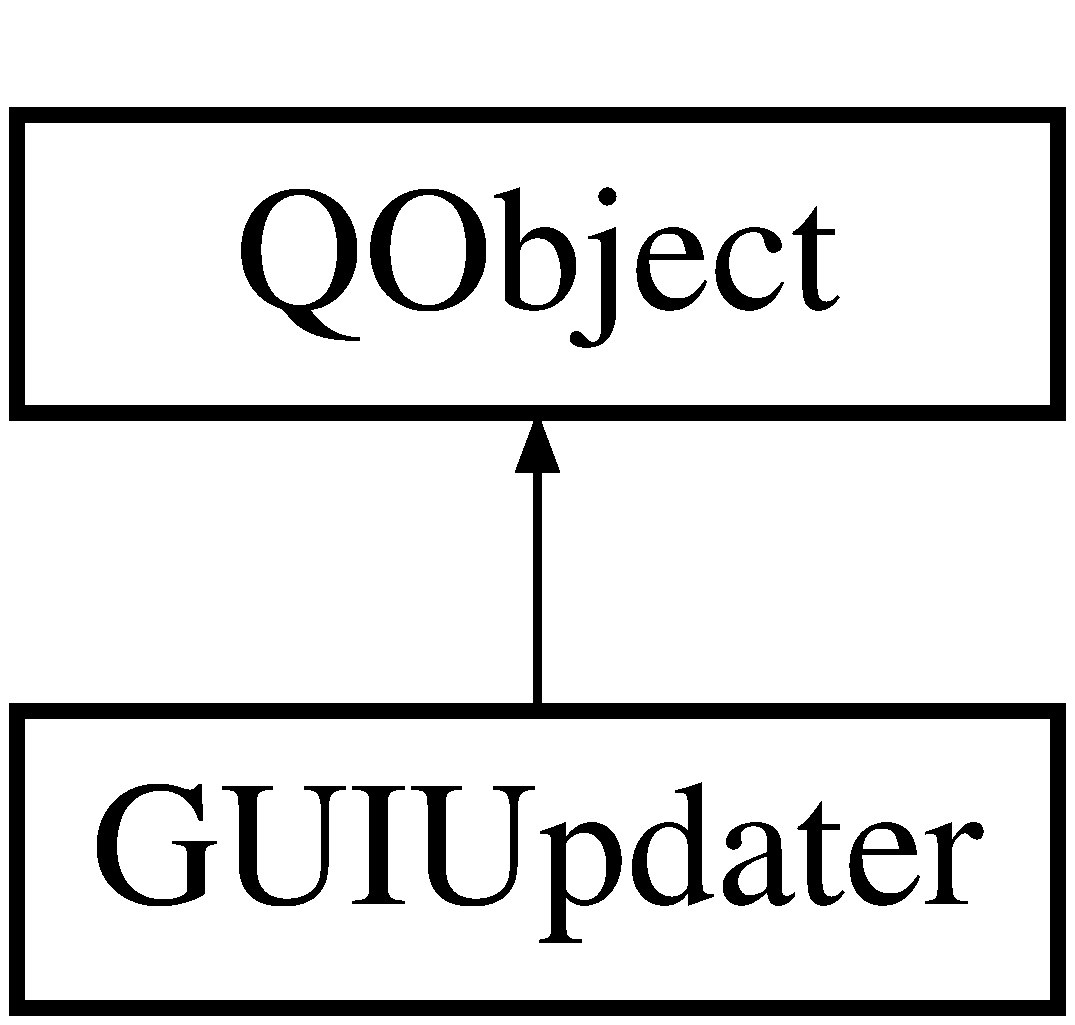
\includegraphics[height=2.000000cm]{class_g_u_i_updater}
\end{center}
\end{figure}
\subsection*{Signals}
\begin{DoxyCompactItemize}
\item 
void {\bfseries update\+Left\+Camera} (const Q\+Image \&)\hypertarget{class_g_u_i_updater_afacf05ece0988f07662eaab5591fd8b7}{}\label{class_g_u_i_updater_afacf05ece0988f07662eaab5591fd8b7}

\item 
void {\bfseries update\+Right\+Camera} (const Q\+Image \&)\hypertarget{class_g_u_i_updater_a1590223624b4a314a9fe56db73d984ab}{}\label{class_g_u_i_updater_a1590223624b4a314a9fe56db73d984ab}

\item 
void {\bfseries do\+Flash} ()\hypertarget{class_g_u_i_updater_ad8113ad71fe2b1cd68b11bf69fc04f95}{}\label{class_g_u_i_updater_ad8113ad71fe2b1cd68b11bf69fc04f95}

\item 
void {\bfseries start\+Calibration} ()\hypertarget{class_g_u_i_updater_a1ab6dfde2b8ea0700d212def0670ab9b}{}\label{class_g_u_i_updater_a1ab6dfde2b8ea0700d212def0670ab9b}

\item 
void {\bfseries start\+Server} ()\hypertarget{class_g_u_i_updater_acc51b4ad134d5972231c4815d6148b83}{}\label{class_g_u_i_updater_acc51b4ad134d5972231c4815d6148b83}

\item 
void {\bfseries pointer\+Detected} ()\hypertarget{class_g_u_i_updater_af4c1cc78e23aa37ff6766be12f45b75f}{}\label{class_g_u_i_updater_af4c1cc78e23aa37ff6766be12f45b75f}

\item 
void {\bfseries pointer\+Not\+Detected} ()\hypertarget{class_g_u_i_updater_a25d97041202cd55c22064b99bddefc5f}{}\label{class_g_u_i_updater_a25d97041202cd55c22064b99bddefc5f}

\end{DoxyCompactItemize}
\subsection*{Public Member Functions}
\begin{DoxyCompactItemize}
\item 
\hyperlink{class_g_u_i_updater_aead8933227b7b7cc78e23b98d6c80ab1}{G\+U\+I\+Updater} (Q\+Object $\ast$parent=0)
\item 
\hyperlink{class_g_u_i_updater_aabcc67dca68b515f3a86caab5f347b8e}{$\sim$\+G\+U\+I\+Updater} ()
\item 
bool \hyperlink{class_g_u_i_updater_af392547bf970784b35f47118512edb0e}{activate\+Cameras} ()
\item 
void \hyperlink{class_g_u_i_updater_a965d3cc548ceb3bfad4dd3be8ddd4e54}{start\+Cameras} ()
\item 
void \hyperlink{class_g_u_i_updater_ae51c4254189ed802733dcf6922851426}{Shut\+Down\+Cameras} ()
\item 
void \hyperlink{class_g_u_i_updater_acf45c3f51346a40e94988d2544650d3b}{Show\+Cameras} ()
\item 
bool \hyperlink{class_g_u_i_updater_abfd0c6a214ab802eaa64e689010cdfeb}{get\+Pointer\+Data} (const std\+::string \&file\+Name)
\item 
void \hyperlink{class_g_u_i_updater_a677be84d397c616cb70d011b127406a5}{get\+Rigids\+Data} ()
\item 
bool \hyperlink{class_g_u_i_updater_abed450cacbd127705c14f797a5c1470d}{calib\+Pointer} ()
\item 
void \hyperlink{class_g_u_i_updater_a978e2b67abc8c081b61a7b0956bcabe4}{set\+Show\+Zone} (bool status)
\item 
void \hyperlink{class_g_u_i_updater_aa0677943be1e52a2852295384034fcd9}{set\+Take\+Snapshot} (bool status)
\item 
void \hyperlink{class_g_u_i_updater_a0646d9ce35c4fdcfc3ffa99c2b795bbe}{set\+Pics2\+Take} (int num\+Pics)
\item 
void \hyperlink{class_g_u_i_updater_ae5ce3b5dc00512e178cd7d7b16596463}{set\+Detect\+Rigids} (bool status)
\item 
void \hyperlink{class_g_u_i_updater_aa938ec821b9be8d1cd953fb0f9cbde5f}{set\+Detect\+Pointer} (bool status)
\item 
void \hyperlink{class_g_u_i_updater_af5e61de316d9cb02a61944319e25f6d1}{set\+Delta} (float delta)
\item 
void \hyperlink{class_g_u_i_updater_a8d47fbed8c4e041cbc91c2e868000e4e}{write\+Matrices} ()
\item 
void \hyperlink{class_g_u_i_updater_ae716caa2ecd78c5fa939f9cb34a0bc48}{set\+Centroid} (cv\+::\+Mat\+\_\+$<$ double $>$ centroid, std\+::string \&bone)
\end{DoxyCompactItemize}


\subsection{Constructor \& Destructor Documentation}
\index{G\+U\+I\+Updater@{G\+U\+I\+Updater}!G\+U\+I\+Updater@{G\+U\+I\+Updater}}
\index{G\+U\+I\+Updater@{G\+U\+I\+Updater}!G\+U\+I\+Updater@{G\+U\+I\+Updater}}
\subsubsection[{\texorpdfstring{G\+U\+I\+Updater(\+Q\+Object $\ast$parent=0)}{GUIUpdater(QObject *parent=0)}}]{\setlength{\rightskip}{0pt plus 5cm}G\+U\+I\+Updater\+::\+G\+U\+I\+Updater (
\begin{DoxyParamCaption}
\item[{Q\+Object $\ast$}]{parent = {\ttfamily 0}}
\end{DoxyParamCaption}
)\hspace{0.3cm}{\ttfamily [explicit]}}\hypertarget{class_g_u_i_updater_aead8933227b7b7cc78e23b98d6c80ab1}{}\label{class_g_u_i_updater_aead8933227b7b7cc78e23b98d6c80ab1}
Constructor por defecto \index{G\+U\+I\+Updater@{G\+U\+I\+Updater}!````~G\+U\+I\+Updater@{$\sim$\+G\+U\+I\+Updater}}
\index{````~G\+U\+I\+Updater@{$\sim$\+G\+U\+I\+Updater}!G\+U\+I\+Updater@{G\+U\+I\+Updater}}
\subsubsection[{\texorpdfstring{$\sim$\+G\+U\+I\+Updater()}{~GUIUpdater()}}]{\setlength{\rightskip}{0pt plus 5cm}G\+U\+I\+Updater\+::$\sim$\+G\+U\+I\+Updater (
\begin{DoxyParamCaption}
{}
\end{DoxyParamCaption}
)}\hypertarget{class_g_u_i_updater_aabcc67dca68b515f3a86caab5f347b8e}{}\label{class_g_u_i_updater_aabcc67dca68b515f3a86caab5f347b8e}
Destructor por defecto 

\subsection{Member Function Documentation}
\index{G\+U\+I\+Updater@{G\+U\+I\+Updater}!activate\+Cameras@{activate\+Cameras}}
\index{activate\+Cameras@{activate\+Cameras}!G\+U\+I\+Updater@{G\+U\+I\+Updater}}
\subsubsection[{\texorpdfstring{activate\+Cameras()}{activateCameras()}}]{\setlength{\rightskip}{0pt plus 5cm}bool G\+U\+I\+Updater\+::activate\+Cameras (
\begin{DoxyParamCaption}
{}
\end{DoxyParamCaption}
)}\hypertarget{class_g_u_i_updater_af392547bf970784b35f47118512edb0e}{}\label{class_g_u_i_updater_af392547bf970784b35f47118512edb0e}
Obtiene una instancia de cada cámaras. \begin{DoxyReturn}{Returns}
verdadero/falso si pudo/no pudo activar las dos cámaras. 
\end{DoxyReturn}
\index{G\+U\+I\+Updater@{G\+U\+I\+Updater}!calib\+Pointer@{calib\+Pointer}}
\index{calib\+Pointer@{calib\+Pointer}!G\+U\+I\+Updater@{G\+U\+I\+Updater}}
\subsubsection[{\texorpdfstring{calib\+Pointer()}{calibPointer()}}]{\setlength{\rightskip}{0pt plus 5cm}bool G\+U\+I\+Updater\+::calib\+Pointer (
\begin{DoxyParamCaption}
{}
\end{DoxyParamCaption}
)}\hypertarget{class_g_u_i_updater_abed450cacbd127705c14f797a5c1470d}{}\label{class_g_u_i_updater_abed450cacbd127705c14f797a5c1470d}
Si detecta el pointer, almacena los puntos barridos en un archivo. También emite señales para indicar si se está detectando o no el pointer en el momento. 
\begin{DoxyParams}{Parameters}
{\em file\+Name} & nombre del archivo. \\
\hline
\end{DoxyParams}
\index{G\+U\+I\+Updater@{G\+U\+I\+Updater}!get\+Pointer\+Data@{get\+Pointer\+Data}}
\index{get\+Pointer\+Data@{get\+Pointer\+Data}!G\+U\+I\+Updater@{G\+U\+I\+Updater}}
\subsubsection[{\texorpdfstring{get\+Pointer\+Data(const std\+::string \&file\+Name)}{getPointerData(const std::string &fileName)}}]{\setlength{\rightskip}{0pt plus 5cm}bool G\+U\+I\+Updater\+::get\+Pointer\+Data (
\begin{DoxyParamCaption}
\item[{const std\+::string \&}]{file\+Name}
\end{DoxyParamCaption}
)}\hypertarget{class_g_u_i_updater_abfd0c6a214ab802eaa64e689010cdfeb}{}\label{class_g_u_i_updater_abfd0c6a214ab802eaa64e689010cdfeb}
Si detecta el pointer, almacena los puntos barridos en un archivo. También emite señales para indicar si se está detectando o no el pointer en el momento. 
\begin{DoxyParams}{Parameters}
{\em file\+Name} & nombre del archivo. \\
\hline
\end{DoxyParams}
\index{G\+U\+I\+Updater@{G\+U\+I\+Updater}!get\+Rigids\+Data@{get\+Rigids\+Data}}
\index{get\+Rigids\+Data@{get\+Rigids\+Data}!G\+U\+I\+Updater@{G\+U\+I\+Updater}}
\subsubsection[{\texorpdfstring{get\+Rigids\+Data()}{getRigidsData()}}]{\setlength{\rightskip}{0pt plus 5cm}void G\+U\+I\+Updater\+::get\+Rigids\+Data (
\begin{DoxyParamCaption}
{}
\end{DoxyParamCaption}
)}\hypertarget{class_g_u_i_updater_a677be84d397c616cb70d011b127406a5}{}\label{class_g_u_i_updater_a677be84d397c616cb70d011b127406a5}
Detecta los rígidos en escena, inicia el servidor y lo utiliza para enviar los datos a la escena de Unity. \index{G\+U\+I\+Updater@{G\+U\+I\+Updater}!set\+Centroid@{set\+Centroid}}
\index{set\+Centroid@{set\+Centroid}!G\+U\+I\+Updater@{G\+U\+I\+Updater}}
\subsubsection[{\texorpdfstring{set\+Centroid(cv\+::\+Mat\+\_\+$<$ double $>$ centroid, std\+::string \&bone)}{setCentroid(cv::Mat_< double > centroid, std::string &bone)}}]{\setlength{\rightskip}{0pt plus 5cm}void G\+U\+I\+Updater\+::set\+Centroid (
\begin{DoxyParamCaption}
\item[{cv\+::\+Mat\+\_\+$<$ double $>$}]{centroid, }
\item[{std\+::string \&}]{bone}
\end{DoxyParamCaption}
)}\hypertarget{class_g_u_i_updater_ae716caa2ecd78c5fa939f9cb34a0bc48}{}\label{class_g_u_i_updater_ae716caa2ecd78c5fa939f9cb34a0bc48}
Asocia las coordendas del centroide de cada uno de los huesos. 
\begin{DoxyParams}{Parameters}
{\em centroid} & coordenadas en 3D del centroide del hueso. \\
\hline
{\em bone} & nombre del hueso al cual se le asociarán las coordenadas. \\
\hline
\end{DoxyParams}
\index{G\+U\+I\+Updater@{G\+U\+I\+Updater}!set\+Delta@{set\+Delta}}
\index{set\+Delta@{set\+Delta}!G\+U\+I\+Updater@{G\+U\+I\+Updater}}
\subsubsection[{\texorpdfstring{set\+Delta(float delta)}{setDelta(float delta)}}]{\setlength{\rightskip}{0pt plus 5cm}void G\+U\+I\+Updater\+::set\+Delta (
\begin{DoxyParamCaption}
\item[{float}]{delta}
\end{DoxyParamCaption}
)}\hypertarget{class_g_u_i_updater_af5e61de316d9cb02a61944319e25f6d1}{}\label{class_g_u_i_updater_af5e61de316d9cb02a61944319e25f6d1}
Setter para delta 
\begin{DoxyParams}{Parameters}
{\em delta} & nuevo estado \\
\hline
\end{DoxyParams}
\index{G\+U\+I\+Updater@{G\+U\+I\+Updater}!set\+Detect\+Pointer@{set\+Detect\+Pointer}}
\index{set\+Detect\+Pointer@{set\+Detect\+Pointer}!G\+U\+I\+Updater@{G\+U\+I\+Updater}}
\subsubsection[{\texorpdfstring{set\+Detect\+Pointer(bool status)}{setDetectPointer(bool status)}}]{\setlength{\rightskip}{0pt plus 5cm}void G\+U\+I\+Updater\+::set\+Detect\+Pointer (
\begin{DoxyParamCaption}
\item[{bool}]{status}
\end{DoxyParamCaption}
)}\hypertarget{class_g_u_i_updater_aa938ec821b9be8d1cd953fb0f9cbde5f}{}\label{class_g_u_i_updater_aa938ec821b9be8d1cd953fb0f9cbde5f}
Setter para detect\+Pointer 
\begin{DoxyParams}{Parameters}
{\em status} & nuevo estado \\
\hline
\end{DoxyParams}
\index{G\+U\+I\+Updater@{G\+U\+I\+Updater}!set\+Detect\+Rigids@{set\+Detect\+Rigids}}
\index{set\+Detect\+Rigids@{set\+Detect\+Rigids}!G\+U\+I\+Updater@{G\+U\+I\+Updater}}
\subsubsection[{\texorpdfstring{set\+Detect\+Rigids(bool status)}{setDetectRigids(bool status)}}]{\setlength{\rightskip}{0pt plus 5cm}void G\+U\+I\+Updater\+::set\+Detect\+Rigids (
\begin{DoxyParamCaption}
\item[{bool}]{status}
\end{DoxyParamCaption}
)}\hypertarget{class_g_u_i_updater_ae5ce3b5dc00512e178cd7d7b16596463}{}\label{class_g_u_i_updater_ae5ce3b5dc00512e178cd7d7b16596463}
Setter para detect\+Rigids 
\begin{DoxyParams}{Parameters}
{\em status} & nuevo estado \\
\hline
\end{DoxyParams}
\index{G\+U\+I\+Updater@{G\+U\+I\+Updater}!set\+Pics2\+Take@{set\+Pics2\+Take}}
\index{set\+Pics2\+Take@{set\+Pics2\+Take}!G\+U\+I\+Updater@{G\+U\+I\+Updater}}
\subsubsection[{\texorpdfstring{set\+Pics2\+Take(int num\+Pics)}{setPics2Take(int numPics)}}]{\setlength{\rightskip}{0pt plus 5cm}void G\+U\+I\+Updater\+::set\+Pics2\+Take (
\begin{DoxyParamCaption}
\item[{int}]{num\+Pics}
\end{DoxyParamCaption}
)}\hypertarget{class_g_u_i_updater_a0646d9ce35c4fdcfc3ffa99c2b795bbe}{}\label{class_g_u_i_updater_a0646d9ce35c4fdcfc3ffa99c2b795bbe}
Setter para Pics2\+Take 
\begin{DoxyParams}{Parameters}
{\em num\+Pics} & número de imágenes \\
\hline
\end{DoxyParams}
\index{G\+U\+I\+Updater@{G\+U\+I\+Updater}!set\+Show\+Zone@{set\+Show\+Zone}}
\index{set\+Show\+Zone@{set\+Show\+Zone}!G\+U\+I\+Updater@{G\+U\+I\+Updater}}
\subsubsection[{\texorpdfstring{set\+Show\+Zone(bool status)}{setShowZone(bool status)}}]{\setlength{\rightskip}{0pt plus 5cm}void G\+U\+I\+Updater\+::set\+Show\+Zone (
\begin{DoxyParamCaption}
\item[{bool}]{status}
\end{DoxyParamCaption}
)}\hypertarget{class_g_u_i_updater_a978e2b67abc8c081b61a7b0956bcabe4}{}\label{class_g_u_i_updater_a978e2b67abc8c081b61a7b0956bcabe4}
Setter para show\+Zone 
\begin{DoxyParams}{Parameters}
{\em status} & nuevo estado \\
\hline
\end{DoxyParams}
\index{G\+U\+I\+Updater@{G\+U\+I\+Updater}!set\+Take\+Snapshot@{set\+Take\+Snapshot}}
\index{set\+Take\+Snapshot@{set\+Take\+Snapshot}!G\+U\+I\+Updater@{G\+U\+I\+Updater}}
\subsubsection[{\texorpdfstring{set\+Take\+Snapshot(bool status)}{setTakeSnapshot(bool status)}}]{\setlength{\rightskip}{0pt plus 5cm}void G\+U\+I\+Updater\+::set\+Take\+Snapshot (
\begin{DoxyParamCaption}
\item[{bool}]{status}
\end{DoxyParamCaption}
)}\hypertarget{class_g_u_i_updater_aa0677943be1e52a2852295384034fcd9}{}\label{class_g_u_i_updater_aa0677943be1e52a2852295384034fcd9}
Setter para take\+Snapshot 
\begin{DoxyParams}{Parameters}
{\em status} & nuevo estado \\
\hline
\end{DoxyParams}
\index{G\+U\+I\+Updater@{G\+U\+I\+Updater}!Show\+Cameras@{Show\+Cameras}}
\index{Show\+Cameras@{Show\+Cameras}!G\+U\+I\+Updater@{G\+U\+I\+Updater}}
\subsubsection[{\texorpdfstring{Show\+Cameras()}{ShowCameras()}}]{\setlength{\rightskip}{0pt plus 5cm}void G\+U\+I\+Updater\+::\+Show\+Cameras (
\begin{DoxyParamCaption}
{}
\end{DoxyParamCaption}
)}\hypertarget{class_g_u_i_updater_acf45c3f51346a40e94988d2544650d3b}{}\label{class_g_u_i_updater_acf45c3f51346a40e94988d2544650d3b}
Envía los frames de cada una de las cámaras a la G\+UI mediante señales y controla la lógica de captura de imágenes. \index{G\+U\+I\+Updater@{G\+U\+I\+Updater}!Shut\+Down\+Cameras@{Shut\+Down\+Cameras}}
\index{Shut\+Down\+Cameras@{Shut\+Down\+Cameras}!G\+U\+I\+Updater@{G\+U\+I\+Updater}}
\subsubsection[{\texorpdfstring{Shut\+Down\+Cameras()}{ShutDownCameras()}}]{\setlength{\rightskip}{0pt plus 5cm}void G\+U\+I\+Updater\+::\+Shut\+Down\+Cameras (
\begin{DoxyParamCaption}
{}
\end{DoxyParamCaption}
)}\hypertarget{class_g_u_i_updater_ae51c4254189ed802733dcf6922851426}{}\label{class_g_u_i_updater_ae51c4254189ed802733dcf6922851426}
Apaga las cámaras adecuadamente. \index{G\+U\+I\+Updater@{G\+U\+I\+Updater}!start\+Cameras@{start\+Cameras}}
\index{start\+Cameras@{start\+Cameras}!G\+U\+I\+Updater@{G\+U\+I\+Updater}}
\subsubsection[{\texorpdfstring{start\+Cameras()}{startCameras()}}]{\setlength{\rightskip}{0pt plus 5cm}void G\+U\+I\+Updater\+::start\+Cameras (
\begin{DoxyParamCaption}
{}
\end{DoxyParamCaption}
)}\hypertarget{class_g_u_i_updater_a965d3cc548ceb3bfad4dd3be8ddd4e54}{}\label{class_g_u_i_updater_a965d3cc548ceb3bfad4dd3be8ddd4e54}
Configura el modo de video de las cámaras (modo Escala de grises) y demás parámetros iniciales (exposición, intensidad y umbral). \index{G\+U\+I\+Updater@{G\+U\+I\+Updater}!write\+Matrices@{write\+Matrices}}
\index{write\+Matrices@{write\+Matrices}!G\+U\+I\+Updater@{G\+U\+I\+Updater}}
\subsubsection[{\texorpdfstring{write\+Matrices()}{writeMatrices()}}]{\setlength{\rightskip}{0pt plus 5cm}void G\+U\+I\+Updater\+::write\+Matrices (
\begin{DoxyParamCaption}
{}
\end{DoxyParamCaption}
)}\hypertarget{class_g_u_i_updater_a8d47fbed8c4e041cbc91c2e868000e4e}{}\label{class_g_u_i_updater_a8d47fbed8c4e041cbc91c2e868000e4e}
Escribe a un archivo las coordenadas de los clavos y los ángulos de estos respecto a los huesos que les corresponden. 

The documentation for this class was generated from the following files\+:\begin{DoxyCompactItemize}
\item 
C\+:/\+Users/eduar\+\_\+000/\+Documents/\+Visual Studio 2015/\+Projects/\+Navar\+Q\+A/\+Navar\+Q\+A/G\+U\+I\+Updater.\+h\item 
C\+:/\+Users/eduar\+\_\+000/\+Documents/\+Visual Studio 2015/\+Projects/\+Navar\+Q\+A/\+Navar\+Q\+A/\+Generated\+Files/\+Debug/moc\+\_\+\+G\+U\+I\+Updater.\+cpp\item 
C\+:/\+Users/eduar\+\_\+000/\+Documents/\+Visual Studio 2015/\+Projects/\+Navar\+Q\+A/\+Navar\+Q\+A/G\+U\+I\+Updater.\+cpp\end{DoxyCompactItemize}

\hypertarget{struct_custom_camera_library_1_1_label}{}\section{Custom\+Camera\+Library\+:\+:Label Struct Reference}
\label{struct_custom_camera_library_1_1_label}\index{Custom\+Camera\+Library\+::\+Label@{Custom\+Camera\+Library\+::\+Label}}


Esta estructura permite ir haciendo un seguimiento de cada uno de los nodos encontrados en proceso de indentificación de los cuerpos rígidos y es utilizada en el momento de identificar los objetos rígidos en escena.  




{\ttfamily \#include $<$detectbr.\+h$>$}

\subsection*{Public Attributes}
\begin{DoxyCompactItemize}
\item 
int \hyperlink{struct_custom_camera_library_1_1_label_ab47ae69658cf38cb404be369acd6b004}{nro}
\item 
int \hyperlink{struct_custom_camera_library_1_1_label_ab2b02b75eea4dbbce1a157e27142019f}{prev}
\item 
float \hyperlink{struct_custom_camera_library_1_1_label_a2c76fc89c6d5ebd560e1081d456052fc}{peso}
\item 
int \hyperlink{struct_custom_camera_library_1_1_label_aee7618e63b0af9f8471c6c666ccb033f}{marca}
\item 
int \hyperlink{struct_custom_camera_library_1_1_label_a6975017853bad717d96e213e22cc0e18}{objR}
\end{DoxyCompactItemize}


\subsection{Detailed Description}
Esta estructura permite ir haciendo un seguimiento de cada uno de los nodos encontrados en proceso de indentificación de los cuerpos rígidos y es utilizada en el momento de identificar los objetos rígidos en escena. 

\subsection{Member Data Documentation}
\index{Custom\+Camera\+Library\+::\+Label@{Custom\+Camera\+Library\+::\+Label}!marca@{marca}}
\index{marca@{marca}!Custom\+Camera\+Library\+::\+Label@{Custom\+Camera\+Library\+::\+Label}}
\subsubsection[{\texorpdfstring{marca}{marca}}]{\setlength{\rightskip}{0pt plus 5cm}Custom\+Camera\+Library\+::\+Label\+::marca}\hypertarget{struct_custom_camera_library_1_1_label_aee7618e63b0af9f8471c6c666ccb033f}{}\label{struct_custom_camera_library_1_1_label_aee7618e63b0af9f8471c6c666ccb033f}
Indica si la esfera ha sido marcada o no. \index{Custom\+Camera\+Library\+::\+Label@{Custom\+Camera\+Library\+::\+Label}!nro@{nro}}
\index{nro@{nro}!Custom\+Camera\+Library\+::\+Label@{Custom\+Camera\+Library\+::\+Label}}
\subsubsection[{\texorpdfstring{nro}{nro}}]{\setlength{\rightskip}{0pt plus 5cm}Custom\+Camera\+Library\+::\+Label\+::nro}\hypertarget{struct_custom_camera_library_1_1_label_ab47ae69658cf38cb404be369acd6b004}{}\label{struct_custom_camera_library_1_1_label_ab47ae69658cf38cb404be369acd6b004}
Contiene el número del nodo. \index{Custom\+Camera\+Library\+::\+Label@{Custom\+Camera\+Library\+::\+Label}!objR@{objR}}
\index{objR@{objR}!Custom\+Camera\+Library\+::\+Label@{Custom\+Camera\+Library\+::\+Label}}
\subsubsection[{\texorpdfstring{objR}{objR}}]{\setlength{\rightskip}{0pt plus 5cm}Custom\+Camera\+Library\+::\+Label\+::objR}\hypertarget{struct_custom_camera_library_1_1_label_a6975017853bad717d96e213e22cc0e18}{}\label{struct_custom_camera_library_1_1_label_a6975017853bad717d96e213e22cc0e18}
Contiene el identificador del objeto rígido al que pertenece. Según la matriz de distancias de entrada; el C.\+R. 1 corresponde a la 1ra fila de la matriz de distancias teóricas y así susecivamente.

Ejemplo de una matriz de distancias\+: \begin{DoxyVerb} Mat_<float> distances = (Mat_<float>(4, 6) <<

     20.05, 29.26, 49.67, 39.82, 49.55, 51.53,     // POINTER

     35.22, 59.15, 25.07, 44.73, 51.63, 54.93,     //FEMUR

     89.74, 107.01, 80.03, 70.26, 103.56, 59.74,   //TIBIA

     64.75, 118.23, 183.64, 55.66, 126.57, 73.28); //GAFAS
\end{DoxyVerb}


cada fila esta formada por las distancias que hay entre cada esfera que forma un cuerpo rígido. Si el objeto rígido no es identificado entonces tendrá valor de -\/1. \begin{DoxySeeAlso}{See also}
Custom\+Camera\+Library\+::distances 

Custom\+Camera\+Library\+::joskstra() 
\end{DoxySeeAlso}
\index{Custom\+Camera\+Library\+::\+Label@{Custom\+Camera\+Library\+::\+Label}!peso@{peso}}
\index{peso@{peso}!Custom\+Camera\+Library\+::\+Label@{Custom\+Camera\+Library\+::\+Label}}
\subsubsection[{\texorpdfstring{peso}{peso}}]{\setlength{\rightskip}{0pt plus 5cm}Custom\+Camera\+Library\+::\+Label\+::peso}\hypertarget{struct_custom_camera_library_1_1_label_a2c76fc89c6d5ebd560e1081d456052fc}{}\label{struct_custom_camera_library_1_1_label_a2c76fc89c6d5ebd560e1081d456052fc}
Distancia del nodo hasta el nodo de referencia. \index{Custom\+Camera\+Library\+::\+Label@{Custom\+Camera\+Library\+::\+Label}!prev@{prev}}
\index{prev@{prev}!Custom\+Camera\+Library\+::\+Label@{Custom\+Camera\+Library\+::\+Label}}
\subsubsection[{\texorpdfstring{prev}{prev}}]{\setlength{\rightskip}{0pt plus 5cm}Custom\+Camera\+Library\+::\+Label\+::prev}\hypertarget{struct_custom_camera_library_1_1_label_ab2b02b75eea4dbbce1a157e27142019f}{}\label{struct_custom_camera_library_1_1_label_ab2b02b75eea4dbbce1a157e27142019f}
Nodo precedente (-\/1 para el nodo inicial). 

The documentation for this struct was generated from the following file\+:\begin{DoxyCompactItemize}
\item 
C\+:/\+Users/eduar\+\_\+000/\+Documents/\+Visual Studio 2015/\+Projects/\+Navar\+Q\+A/\+Navar\+Q\+A/detectbr.\+h\end{DoxyCompactItemize}

\hypertarget{class_custom_camera_library_1_1_marker}{}\section{Custom\+Camera\+Library\+:\+:Marker Class Reference}
\label{class_custom_camera_library_1_1_marker}\index{Custom\+Camera\+Library\+::\+Marker@{Custom\+Camera\+Library\+::\+Marker}}


{\ttfamily \#include $<$marker.\+h$>$}

\subsection*{Public Member Functions}
\begin{DoxyCompactItemize}
\item 
\hyperlink{class_custom_camera_library_1_1_marker_ad4e167fa334fbde49f073e4362c4d3db}{Marker} ()
\item 
\hyperlink{class_custom_camera_library_1_1_marker_ac34f00758cfb07bcf550209083633eb6}{$\sim$\+Marker} (void)
\item 
\hyperlink{class_custom_camera_library_1_1_marker_af2d2ffcc36c375af9138c1ce65751361}{Marker} (string name)
\item 
double \hyperlink{class_custom_camera_library_1_1_marker_a531c9ce7513ee80a7e6c226840d81463}{Marker\+::getY} ()
\item 
double \hyperlink{class_custom_camera_library_1_1_marker_af6e5dd7cd6e768429e8dcd768042f208}{Marker\+::getX} ()
\item 
void \hyperlink{class_custom_camera_library_1_1_marker_ac7413e8da227e4e5551166ee7981f27a}{Marker\+::setX} (float x)
\item 
void \hyperlink{class_custom_camera_library_1_1_marker_a9ccca6aac23f01511539d9f9e1f874b8}{Marker\+::setY} (float y)
\item 
string \hyperlink{class_custom_camera_library_1_1_marker_a66beaaf58401fcbc9f69530aa23fe87f}{get\+Type} ()
\item 
void \hyperlink{class_custom_camera_library_1_1_marker_accb27bc1a4d0edc55571b6f29af41f4c}{set\+Type} (string t)
\item 
Scalar \hyperlink{class_custom_camera_library_1_1_marker_a4a9365c66d784ec641f36038ce0c1aa4}{get\+Color} ()
\item 
void \hyperlink{class_custom_camera_library_1_1_marker_a7433a7e4ab0bef65ad5987a81d984307}{set\+Color} (Scalar c)
\item 
void \hyperlink{class_custom_camera_library_1_1_marker_a39e4057984377e2dd2fa772dc2816b48}{set\+Area} (float a)
\item 
double \hyperlink{class_custom_camera_library_1_1_marker_a80e3a9409ad839045f9b6481c2334dce}{get\+Area} ()
\end{DoxyCompactItemize}


\subsection{Detailed Description}
Clase que representa un marcador reflectivo. Cuenta con propiedades que la definen y permite ir representando los marcadores que se encuentran dentro de la escena. 

\subsection{Constructor \& Destructor Documentation}
\index{Custom\+Camera\+Library\+::\+Marker@{Custom\+Camera\+Library\+::\+Marker}!Marker@{Marker}}
\index{Marker@{Marker}!Custom\+Camera\+Library\+::\+Marker@{Custom\+Camera\+Library\+::\+Marker}}
\subsubsection[{\texorpdfstring{Marker()}{Marker()}}]{\setlength{\rightskip}{0pt plus 5cm}Marker\+::\+Marker (
\begin{DoxyParamCaption}
{}
\end{DoxyParamCaption}
)}\hypertarget{class_custom_camera_library_1_1_marker_ad4e167fa334fbde49f073e4362c4d3db}{}\label{class_custom_camera_library_1_1_marker_ad4e167fa334fbde49f073e4362c4d3db}
Constructor por omisión. Establece \char`\"{}\+Marker\char`\"{} como tipo para cada marcador (solo es una etiqueta). \index{Custom\+Camera\+Library\+::\+Marker@{Custom\+Camera\+Library\+::\+Marker}!````~Marker@{$\sim$\+Marker}}
\index{````~Marker@{$\sim$\+Marker}!Custom\+Camera\+Library\+::\+Marker@{Custom\+Camera\+Library\+::\+Marker}}
\subsubsection[{\texorpdfstring{$\sim$\+Marker(void)}{~Marker(void)}}]{\setlength{\rightskip}{0pt plus 5cm}Marker\+::$\sim$\+Marker (
\begin{DoxyParamCaption}
\item[{void}]{}
\end{DoxyParamCaption}
)}\hypertarget{class_custom_camera_library_1_1_marker_ac34f00758cfb07bcf550209083633eb6}{}\label{class_custom_camera_library_1_1_marker_ac34f00758cfb07bcf550209083633eb6}
Destructor por omisión. \index{Custom\+Camera\+Library\+::\+Marker@{Custom\+Camera\+Library\+::\+Marker}!Marker@{Marker}}
\index{Marker@{Marker}!Custom\+Camera\+Library\+::\+Marker@{Custom\+Camera\+Library\+::\+Marker}}
\subsubsection[{\texorpdfstring{Marker(string name)}{Marker(string name)}}]{\setlength{\rightskip}{0pt plus 5cm}Custom\+Camera\+Library\+::\+Marker\+::\+Marker (
\begin{DoxyParamCaption}
\item[{string}]{name}
\end{DoxyParamCaption}
)}\hypertarget{class_custom_camera_library_1_1_marker_af2d2ffcc36c375af9138c1ce65751361}{}\label{class_custom_camera_library_1_1_marker_af2d2ffcc36c375af9138c1ce65751361}
Constructor con parámetros. Utilizado si se quiere asignar un nombre distinto al por omisión a los marcadores. 
\begin{DoxyParams}{Parameters}
{\em name} & es el mombre que se le quiere dar a un marcador. (No utilizada por el momento) \\
\hline
\end{DoxyParams}


\subsection{Member Function Documentation}
\index{Custom\+Camera\+Library\+::\+Marker@{Custom\+Camera\+Library\+::\+Marker}!get\+Area@{get\+Area}}
\index{get\+Area@{get\+Area}!Custom\+Camera\+Library\+::\+Marker@{Custom\+Camera\+Library\+::\+Marker}}
\subsubsection[{\texorpdfstring{get\+Area()}{getArea()}}]{\setlength{\rightskip}{0pt plus 5cm}double Custom\+Camera\+Library\+::\+Marker\+::get\+Area (
\begin{DoxyParamCaption}
{}
\end{DoxyParamCaption}
)\hspace{0.3cm}{\ttfamily [inline]}}\hypertarget{class_custom_camera_library_1_1_marker_a80e3a9409ad839045f9b6481c2334dce}{}\label{class_custom_camera_library_1_1_marker_a80e3a9409ad839045f9b6481c2334dce}
Utilizado para obtener el área de un marcador que se ha detectado. \begin{DoxyReturn}{Returns}
el área del marcador. 
\end{DoxyReturn}
\index{Custom\+Camera\+Library\+::\+Marker@{Custom\+Camera\+Library\+::\+Marker}!get\+Color@{get\+Color}}
\index{get\+Color@{get\+Color}!Custom\+Camera\+Library\+::\+Marker@{Custom\+Camera\+Library\+::\+Marker}}
\subsubsection[{\texorpdfstring{get\+Color()}{getColor()}}]{\setlength{\rightskip}{0pt plus 5cm}Scalar Custom\+Camera\+Library\+::\+Marker\+::get\+Color (
\begin{DoxyParamCaption}
{}
\end{DoxyParamCaption}
)\hspace{0.3cm}{\ttfamily [inline]}}\hypertarget{class_custom_camera_library_1_1_marker_a4a9365c66d784ec641f36038ce0c1aa4}{}\label{class_custom_camera_library_1_1_marker_a4a9365c66d784ec641f36038ce0c1aa4}
Obtiene el color que se le ha indicado al marcador, el color es utilizado para indicar de qué color son los marcadores (El \char`\"{}color\char`\"{} es asignado desde el constructor). \begin{DoxyReturn}{Returns}
el color del marcador. 
\end{DoxyReturn}
\index{Custom\+Camera\+Library\+::\+Marker@{Custom\+Camera\+Library\+::\+Marker}!get\+Type@{get\+Type}}
\index{get\+Type@{get\+Type}!Custom\+Camera\+Library\+::\+Marker@{Custom\+Camera\+Library\+::\+Marker}}
\subsubsection[{\texorpdfstring{get\+Type()}{getType()}}]{\setlength{\rightskip}{0pt plus 5cm}string Custom\+Camera\+Library\+::\+Marker\+::get\+Type (
\begin{DoxyParamCaption}
{}
\end{DoxyParamCaption}
)\hspace{0.3cm}{\ttfamily [inline]}}\hypertarget{class_custom_camera_library_1_1_marker_a66beaaf58401fcbc9f69530aa23fe87f}{}\label{class_custom_camera_library_1_1_marker_a66beaaf58401fcbc9f69530aa23fe87f}
Obtiene el \char`\"{}tipo\char`\"{} que se le haya colocado a los marcadores (El \char`\"{}tipo\char`\"{} es asignado desde el constructor). \begin{DoxyReturn}{Returns}
un string que almacena el nombre de los marcadores. 
\end{DoxyReturn}
\index{Custom\+Camera\+Library\+::\+Marker@{Custom\+Camera\+Library\+::\+Marker}!Marker\+::getX@{Marker\+::getX}}
\index{Marker\+::getX@{Marker\+::getX}!Custom\+Camera\+Library\+::\+Marker@{Custom\+Camera\+Library\+::\+Marker}}
\subsubsection[{\texorpdfstring{Marker\+::get\+X()}{Marker::getX()}}]{\setlength{\rightskip}{0pt plus 5cm}double Custom\+Camera\+Library\+::\+Marker\+::\+Marker\+::getX (
\begin{DoxyParamCaption}
{}
\end{DoxyParamCaption}
)\hspace{0.3cm}{\ttfamily [inline]}}\hypertarget{class_custom_camera_library_1_1_marker_af6e5dd7cd6e768429e8dcd768042f208}{}\label{class_custom_camera_library_1_1_marker_af6e5dd7cd6e768429e8dcd768042f208}
Devuelve la posición {\itshape X} en pixeles de un marcador. \begin{DoxyReturn}{Returns}
la posición {\itshape X} en pixeles de un marcador 
\end{DoxyReturn}
\index{Custom\+Camera\+Library\+::\+Marker@{Custom\+Camera\+Library\+::\+Marker}!Marker\+::getY@{Marker\+::getY}}
\index{Marker\+::getY@{Marker\+::getY}!Custom\+Camera\+Library\+::\+Marker@{Custom\+Camera\+Library\+::\+Marker}}
\subsubsection[{\texorpdfstring{Marker\+::get\+Y()}{Marker::getY()}}]{\setlength{\rightskip}{0pt plus 5cm}double Custom\+Camera\+Library\+::\+Marker\+::\+Marker\+::getY (
\begin{DoxyParamCaption}
{}
\end{DoxyParamCaption}
)\hspace{0.3cm}{\ttfamily [inline]}}\hypertarget{class_custom_camera_library_1_1_marker_a531c9ce7513ee80a7e6c226840d81463}{}\label{class_custom_camera_library_1_1_marker_a531c9ce7513ee80a7e6c226840d81463}
Devuelve la posición {\itshape Y} en pixeles de un marcador. \begin{DoxyReturn}{Returns}
la posición {\itshape Y} en pixeles de un marcador 
\end{DoxyReturn}
\index{Custom\+Camera\+Library\+::\+Marker@{Custom\+Camera\+Library\+::\+Marker}!Marker\+::setX@{Marker\+::setX}}
\index{Marker\+::setX@{Marker\+::setX}!Custom\+Camera\+Library\+::\+Marker@{Custom\+Camera\+Library\+::\+Marker}}
\subsubsection[{\texorpdfstring{Marker\+::set\+X(float x)}{Marker::setX(float x)}}]{\setlength{\rightskip}{0pt plus 5cm}void Custom\+Camera\+Library\+::\+Marker\+::\+Marker\+::setX (
\begin{DoxyParamCaption}
\item[{float}]{x}
\end{DoxyParamCaption}
)\hspace{0.3cm}{\ttfamily [inline]}}\hypertarget{class_custom_camera_library_1_1_marker_ac7413e8da227e4e5551166ee7981f27a}{}\label{class_custom_camera_library_1_1_marker_ac7413e8da227e4e5551166ee7981f27a}
Establece la posición {\itshape X} de un marcador detectado en la escena. 
\begin{DoxyParams}{Parameters}
{\em x} & un número que indica la posición en {\itshape X} en pixeles. \\
\hline
\end{DoxyParams}
\index{Custom\+Camera\+Library\+::\+Marker@{Custom\+Camera\+Library\+::\+Marker}!Marker\+::setY@{Marker\+::setY}}
\index{Marker\+::setY@{Marker\+::setY}!Custom\+Camera\+Library\+::\+Marker@{Custom\+Camera\+Library\+::\+Marker}}
\subsubsection[{\texorpdfstring{Marker\+::set\+Y(float y)}{Marker::setY(float y)}}]{\setlength{\rightskip}{0pt plus 5cm}void Custom\+Camera\+Library\+::\+Marker\+::\+Marker\+::setY (
\begin{DoxyParamCaption}
\item[{float}]{y}
\end{DoxyParamCaption}
)\hspace{0.3cm}{\ttfamily [inline]}}\hypertarget{class_custom_camera_library_1_1_marker_a9ccca6aac23f01511539d9f9e1f874b8}{}\label{class_custom_camera_library_1_1_marker_a9ccca6aac23f01511539d9f9e1f874b8}
Establece la posición {\itshape Y} de un marcador detectado en la escena. 
\begin{DoxyParams}{Parameters}
{\em y} & un número que indica la posición en {\itshape Y} en pixeles. \\
\hline
\end{DoxyParams}
\index{Custom\+Camera\+Library\+::\+Marker@{Custom\+Camera\+Library\+::\+Marker}!set\+Area@{set\+Area}}
\index{set\+Area@{set\+Area}!Custom\+Camera\+Library\+::\+Marker@{Custom\+Camera\+Library\+::\+Marker}}
\subsubsection[{\texorpdfstring{set\+Area(float a)}{setArea(float a)}}]{\setlength{\rightskip}{0pt plus 5cm}void Custom\+Camera\+Library\+::\+Marker\+::set\+Area (
\begin{DoxyParamCaption}
\item[{float}]{a}
\end{DoxyParamCaption}
)\hspace{0.3cm}{\ttfamily [inline]}}\hypertarget{class_custom_camera_library_1_1_marker_a39e4057984377e2dd2fa772dc2816b48}{}\label{class_custom_camera_library_1_1_marker_a39e4057984377e2dd2fa772dc2816b48}
Utilizado para guardar el área de un marcador que se ha detectado. 
\begin{DoxyParams}{Parameters}
{\em a} & área del marcador. \\
\hline
\end{DoxyParams}
\index{Custom\+Camera\+Library\+::\+Marker@{Custom\+Camera\+Library\+::\+Marker}!set\+Color@{set\+Color}}
\index{set\+Color@{set\+Color}!Custom\+Camera\+Library\+::\+Marker@{Custom\+Camera\+Library\+::\+Marker}}
\subsubsection[{\texorpdfstring{set\+Color(\+Scalar c)}{setColor(Scalar c)}}]{\setlength{\rightskip}{0pt plus 5cm}void Custom\+Camera\+Library\+::\+Marker\+::set\+Color (
\begin{DoxyParamCaption}
\item[{Scalar}]{c}
\end{DoxyParamCaption}
)\hspace{0.3cm}{\ttfamily [inline]}}\hypertarget{class_custom_camera_library_1_1_marker_a7433a7e4ab0bef65ad5987a81d984307}{}\label{class_custom_camera_library_1_1_marker_a7433a7e4ab0bef65ad5987a81d984307}
Asigna el color que tendrán los marcadores, el color es utilizado para indicar de qué color son los marcadores (El \char`\"{}color\char`\"{} es asignado desde el constructor). 
\begin{DoxyParams}{Parameters}
{\em c} & un color para el marcador. \\
\hline
\end{DoxyParams}
\index{Custom\+Camera\+Library\+::\+Marker@{Custom\+Camera\+Library\+::\+Marker}!set\+Type@{set\+Type}}
\index{set\+Type@{set\+Type}!Custom\+Camera\+Library\+::\+Marker@{Custom\+Camera\+Library\+::\+Marker}}
\subsubsection[{\texorpdfstring{set\+Type(string t)}{setType(string t)}}]{\setlength{\rightskip}{0pt plus 5cm}void Custom\+Camera\+Library\+::\+Marker\+::set\+Type (
\begin{DoxyParamCaption}
\item[{string}]{t}
\end{DoxyParamCaption}
)\hspace{0.3cm}{\ttfamily [inline]}}\hypertarget{class_custom_camera_library_1_1_marker_accb27bc1a4d0edc55571b6f29af41f4c}{}\label{class_custom_camera_library_1_1_marker_accb27bc1a4d0edc55571b6f29af41f4c}
Obtiene el \char`\"{}tipo\char`\"{} que se le haya colocado a los marcadores un nombre a los marcadores detectados . 
\begin{DoxyParams}{Parameters}
{\em t} & un número que indica la posición en {\itshape Y} en pixeles. \\
\hline
\end{DoxyParams}


The documentation for this class was generated from the following files\+:\begin{DoxyCompactItemize}
\item 
C\+:/\+Users/eduar\+\_\+000/\+Documents/\+Visual Studio 2015/\+Projects/\+Navar\+Q\+A/\+Navar\+Q\+A/marker.\+h\item 
C\+:/\+Users/eduar\+\_\+000/\+Documents/\+Visual Studio 2015/\+Projects/\+Navar\+Q\+A/\+Navar\+Q\+A/marker.\+cpp\end{DoxyCompactItemize}

\hypertarget{class_n_a_t_utils}{}\section{N\+A\+T\+Utils Class Reference}
\label{class_n_a_t_utils}\index{N\+A\+T\+Utils@{N\+A\+T\+Utils}}
\subsection*{Static Public Member Functions}
\begin{DoxyCompactItemize}
\item 
static int {\bfseries Get\+Local\+I\+P\+Addresses} (unsigned long Addresses\mbox{[}$\,$\mbox{]}, int n\+Max)\hypertarget{class_n_a_t_utils_ae555d6ef00b1390a4a69ee677c8a97f1}{}\label{class_n_a_t_utils_ae555d6ef00b1390a4a69ee677c8a97f1}

\item 
static int {\bfseries Get\+Local\+I\+P\+Addresses2} (unsigned long Addresses\mbox{[}$\,$\mbox{]}, int n\+Max)\hypertarget{class_n_a_t_utils_aeaa1337aa84cffe493d53fdcd809eff7}{}\label{class_n_a_t_utils_aeaa1337aa84cffe493d53fdcd809eff7}

\item 
{\footnotesize template$<$typename T $>$ }\\static void \hyperlink{class_n_a_t_utils_a1786ab9e713ac59587dbe6050d8b91fc}{Qaternion\+To\+Rotation\+Matrix} (T $\ast$q, T $\ast$m)
\begin{DoxyCompactList}\small\item\em Converts a quaternion to a rotation matrix. \end{DoxyCompactList}\item 
{\footnotesize template$<$typename T $>$ }\\static void \hyperlink{class_n_a_t_utils_a825d3061e86f9ac7323935786e8d6c73}{Vec3\+Matrix\+Mult} (T $\ast$v, T $\ast$m)
\begin{DoxyCompactList}\small\item\em Multiplies a vector with 3 components by a 3 x 3 matrix and overwrites the input vector with the result. \end{DoxyCompactList}\item 
static float \hyperlink{class_n_a_t_utils_a2abf69f59abce23991c399d9775cec5a}{Radians\+To\+Degrees} (float f\+Radians)
\begin{DoxyCompactList}\small\item\em Converts radians to degrees. \end{DoxyCompactList}\end{DoxyCompactItemize}


\subsection{Member Function Documentation}
\index{N\+A\+T\+Utils@{N\+A\+T\+Utils}!Qaternion\+To\+Rotation\+Matrix@{Qaternion\+To\+Rotation\+Matrix}}
\index{Qaternion\+To\+Rotation\+Matrix@{Qaternion\+To\+Rotation\+Matrix}!N\+A\+T\+Utils@{N\+A\+T\+Utils}}
\subsubsection[{\texorpdfstring{Qaternion\+To\+Rotation\+Matrix(\+T $\ast$q, T $\ast$m)}{QaternionToRotationMatrix(T *q, T *m)}}]{\setlength{\rightskip}{0pt plus 5cm}template$<$typename T $>$ void N\+A\+T\+Utils\+::\+Qaternion\+To\+Rotation\+Matrix (
\begin{DoxyParamCaption}
\item[{T $\ast$}]{q, }
\item[{T $\ast$}]{m}
\end{DoxyParamCaption}
)\hspace{0.3cm}{\ttfamily [static]}}\hypertarget{class_n_a_t_utils_a1786ab9e713ac59587dbe6050d8b91fc}{}\label{class_n_a_t_utils_a1786ab9e713ac59587dbe6050d8b91fc}


Converts a quaternion to a rotation matrix. 


\begin{DoxyParams}{Parameters}
{\em q} & Quaternion stored in x, y, z, w order.\\
\hline
{\em m} & Pointer to an array of length 9. Rotation matrix is placed into this array in column major order.\\
\hline
\end{DoxyParams}
\index{N\+A\+T\+Utils@{N\+A\+T\+Utils}!Radians\+To\+Degrees@{Radians\+To\+Degrees}}
\index{Radians\+To\+Degrees@{Radians\+To\+Degrees}!N\+A\+T\+Utils@{N\+A\+T\+Utils}}
\subsubsection[{\texorpdfstring{Radians\+To\+Degrees(float f\+Radians)}{RadiansToDegrees(float fRadians)}}]{\setlength{\rightskip}{0pt plus 5cm}static float N\+A\+T\+Utils\+::\+Radians\+To\+Degrees (
\begin{DoxyParamCaption}
\item[{float}]{f\+Radians}
\end{DoxyParamCaption}
)\hspace{0.3cm}{\ttfamily [inline]}, {\ttfamily [static]}}\hypertarget{class_n_a_t_utils_a2abf69f59abce23991c399d9775cec5a}{}\label{class_n_a_t_utils_a2abf69f59abce23991c399d9775cec5a}


Converts radians to degrees. 


\begin{DoxyParams}{Parameters}
{\em f\+Radians} & Radians.\\
\hline
\end{DoxyParams}
\begin{DoxyReturn}{Returns}
Degrees.
\end{DoxyReturn}
\index{N\+A\+T\+Utils@{N\+A\+T\+Utils}!Vec3\+Matrix\+Mult@{Vec3\+Matrix\+Mult}}
\index{Vec3\+Matrix\+Mult@{Vec3\+Matrix\+Mult}!N\+A\+T\+Utils@{N\+A\+T\+Utils}}
\subsubsection[{\texorpdfstring{Vec3\+Matrix\+Mult(\+T $\ast$v, T $\ast$m)}{Vec3MatrixMult(T *v, T *m)}}]{\setlength{\rightskip}{0pt plus 5cm}template$<$typename T $>$ void N\+A\+T\+Utils\+::\+Vec3\+Matrix\+Mult (
\begin{DoxyParamCaption}
\item[{T $\ast$}]{v, }
\item[{T $\ast$}]{m}
\end{DoxyParamCaption}
)\hspace{0.3cm}{\ttfamily [static]}}\hypertarget{class_n_a_t_utils_a825d3061e86f9ac7323935786e8d6c73}{}\label{class_n_a_t_utils_a825d3061e86f9ac7323935786e8d6c73}


Multiplies a vector with 3 components by a 3 x 3 matrix and overwrites the input vector with the result. 


\begin{DoxyParams}{Parameters}
{\em v} & On input a vector with 3 components. On output the result of the multiplication.\\
\hline
{\em m} & 3 x 3 matrix stored in column major order\\
\hline
\end{DoxyParams}


The documentation for this class was generated from the following files\+:\begin{DoxyCompactItemize}
\item 
C\+:/\+Users/eduar\+\_\+000/\+Documents/\+Visual Studio 2015/\+Projects/\+Navar\+Q\+A/\+Navar\+Q\+A/N\+A\+T\+Utils.\+h\item 
C\+:/\+Users/eduar\+\_\+000/\+Documents/\+Visual Studio 2015/\+Projects/\+Navar\+Q\+A/\+Navar\+Q\+A/N\+A\+T\+Utils.\+cpp\end{DoxyCompactItemize}

\hypertarget{class_navar_q_t}{}\section{Navar\+QT Class Reference}
\label{class_navar_q_t}\index{Navar\+QT@{Navar\+QT}}
Inheritance diagram for Navar\+QT\+:\begin{figure}[H]
\begin{center}
\leavevmode
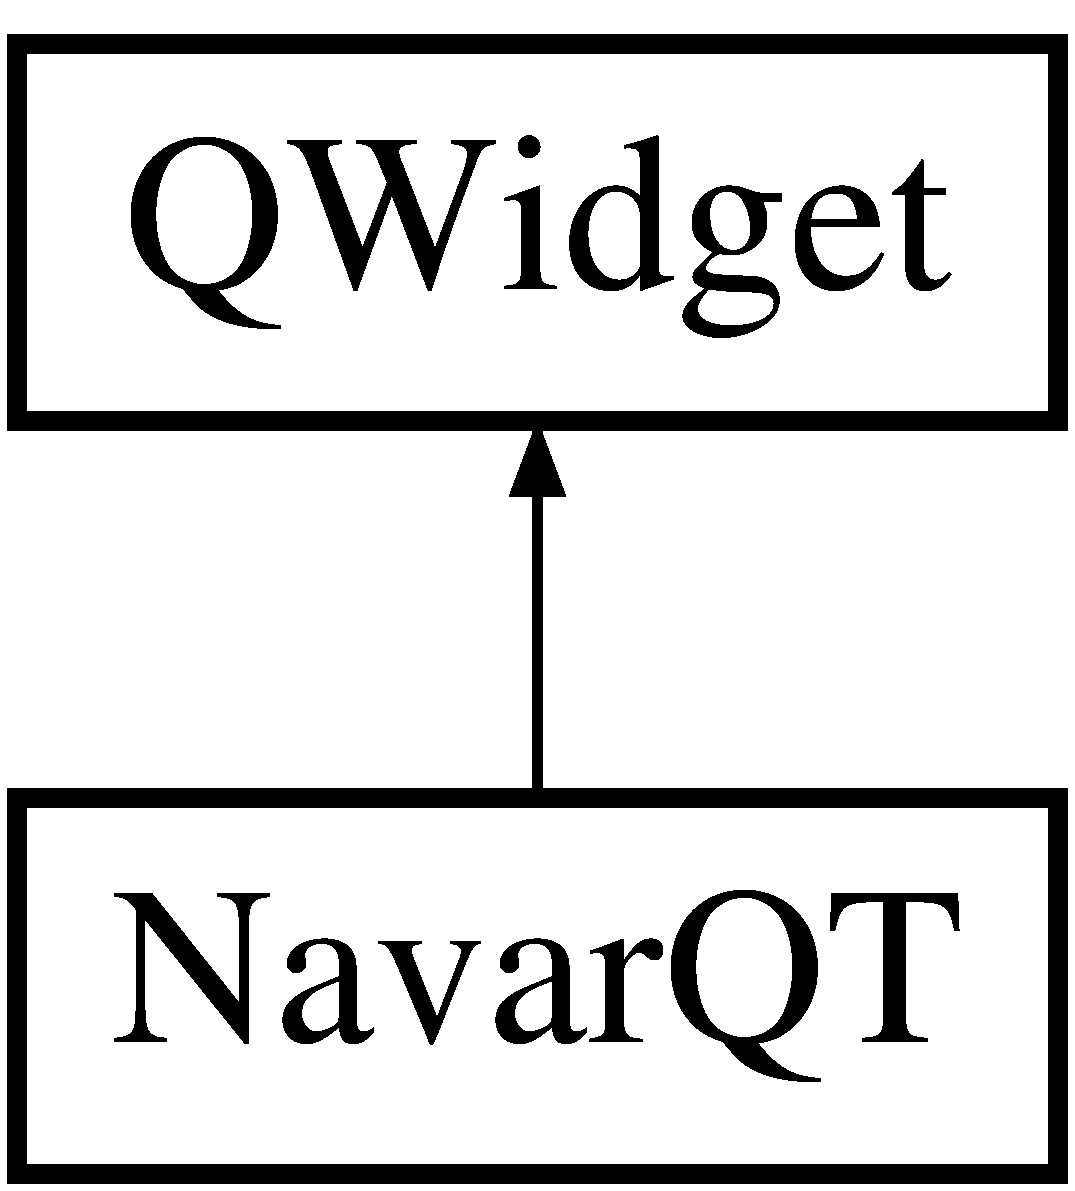
\includegraphics[height=2.000000cm]{class_navar_q_t}
\end{center}
\end{figure}
\subsection*{Public Slots}
\begin{DoxyCompactItemize}
\item 
void \hyperlink{class_navar_q_t_a7f799a993f8d49a3fa6fce6a6c135a93}{create\+Label\+Left} (const Q\+Image \&img\+Source)
\item 
void \hyperlink{class_navar_q_t_a83e8f4a43dd2f68211e7cc98288871ba}{create\+Label\+Right} (const Q\+Image \&img\+Source)
\item 
void \hyperlink{class_navar_q_t_a57c443ce462d7197270723af949db1ae}{start\+Calibration} ()
\item 
void \hyperlink{class_navar_q_t_a14efead4ef08a35f964ae492a6f44fff}{start\+Server} ()
\item 
void \hyperlink{class_navar_q_t_abbd46683ba8e1eb5332f6d0bdf3267ca}{color\+Label\+Green} ()
\item 
void \hyperlink{class_navar_q_t_acaf2fc30199555904840a65e431e3f5a}{color\+Label\+Red} ()
\item 
void \hyperlink{class_navar_q_t_a275c4ff527e4788362338b632cf682ea}{do\+Flash} ()
\item 
void \hyperlink{class_navar_q_t_ae671c9a7db680ac6770f7d86c6854776}{on\+\_\+push\+Button\+\_\+1\+\_\+clicked} ()
\item 
void \hyperlink{class_navar_q_t_ac2f9730b97ead61c3cf37e8320ca0342}{on\+\_\+push\+Button\+\_\+2\+\_\+clicked} ()
\item 
void \hyperlink{class_navar_q_t_a977bf47e535b6c0acedeac1437e0fba7}{on\+\_\+push\+Button\+\_\+3\+\_\+clicked} ()
\item 
void \hyperlink{class_navar_q_t_ab91fa0636ab3a585a2bf7422e4f2b5d8}{on\+\_\+push\+Button\+\_\+4\+\_\+clicked} ()
\item 
void \hyperlink{class_navar_q_t_a1e10f125024be99c20d90e36949b9269}{on\+\_\+push\+Button\+\_\+5\+\_\+clicked} ()
\item 
void \hyperlink{class_navar_q_t_a99198b6fbaa784379dcaa68e2448359d}{on\+\_\+push\+Button\+\_\+6\+\_\+clicked} ()
\item 
void \hyperlink{class_navar_q_t_a3486dd54514c0c5cc5b618f29f233795}{on\+\_\+push\+Button\+\_\+7\+\_\+clicked} ()
\item 
void \hyperlink{class_navar_q_t_a13c92a1f5bc243854fcbb4670e898e30}{on\+\_\+push\+Button\+\_\+8\+\_\+clicked} ()
\item 
void \hyperlink{class_navar_q_t_ac9c2e8d4b9be1a96a292576090fd8350}{on\+\_\+push\+Button\+\_\+9\+\_\+clicked} ()
\item 
void \hyperlink{class_navar_q_t_a80e48ff9d9ac6b7eaccb1d348ed51a94}{on\+\_\+push\+Button\+\_\+10\+\_\+clicked} ()
\item 
void \hyperlink{class_navar_q_t_af7f07042a8270fb922050c93d05be8da}{on\+\_\+push\+Button\+\_\+close\+\_\+clicked} ()
\item 
void \hyperlink{class_navar_q_t_a10e80fed3a4224a006faddd9e41a68ae}{on\+\_\+push\+Button\+\_\+tibia\+\_\+clicked} ()
\item 
void \hyperlink{class_navar_q_t_a2bcee87b6a929f73c8b692296dfe1cd1}{on\+\_\+push\+Button\+\_\+femur\+\_\+clicked} ()
\item 
void \hyperlink{class_navar_q_t_ad515aba34a9e85018b34649087c09cb4}{on\+\_\+push\+Button\+\_\+step\+\_\+1\+\_\+clicked} ()
\item 
void \hyperlink{class_navar_q_t_a99e83586d65bd2ba3cee8a91bad1026c}{on\+\_\+push\+Button\+\_\+step\+\_\+2\+\_\+clicked} ()
\item 
void \hyperlink{class_navar_q_t_a4c46f2e45aa7054ec7285d35712000c6}{on\+\_\+push\+Button\+\_\+step\+\_\+3\+\_\+clicked} ()
\item 
void \hyperlink{class_navar_q_t_a764d70a919e3401eaf9b054ffaae2cf2}{on\+\_\+push\+Button\+\_\+step\+\_\+4\+\_\+clicked} ()
\end{DoxyCompactItemize}
\subsection*{Public Member Functions}
\begin{DoxyCompactItemize}
\item 
\hyperlink{class_navar_q_t_a7b78cbb0e488599ea015975711b98787}{Navar\+QT} (Q\+Widget $\ast$parent=0)
\end{DoxyCompactItemize}
\subsection*{Public Attributes}
\begin{DoxyCompactItemize}
\item 
Q\+Pointer$<$ Q\+Thread $>$ {\bfseries thread}\hypertarget{class_navar_q_t_a0d3de848e8252607ecbf90097a449aed}{}\label{class_navar_q_t_a0d3de848e8252607ecbf90097a449aed}

\item 
Q\+Pointer$<$ \hyperlink{class_g_u_i_updater}{G\+U\+I\+Updater} $>$ {\bfseries updater}\hypertarget{class_navar_q_t_a0cfefb0d249de963c6b36254509858d1}{}\label{class_navar_q_t_a0cfefb0d249de963c6b36254509858d1}

\item 
Q\+Pointer$<$ Q\+Process $>$ {\bfseries process\+\_\+rigids}\hypertarget{class_navar_q_t_aa74e1d7923fc1389c067699863f8aa18}{}\label{class_navar_q_t_aa74e1d7923fc1389c067699863f8aa18}

\item 
Q\+Pointer$<$ Q\+Process $>$ {\bfseries process\+\_\+client}\hypertarget{class_navar_q_t_a2a265b40387a374e15d485a91c84eff7}{}\label{class_navar_q_t_a2a265b40387a374e15d485a91c84eff7}

\end{DoxyCompactItemize}


\subsection{Constructor \& Destructor Documentation}
\index{Navar\+QT@{Navar\+QT}!Navar\+QT@{Navar\+QT}}
\index{Navar\+QT@{Navar\+QT}!Navar\+QT@{Navar\+QT}}
\subsubsection[{\texorpdfstring{Navar\+Q\+T(\+Q\+Widget $\ast$parent=0)}{NavarQT(QWidget *parent=0)}}]{\setlength{\rightskip}{0pt plus 5cm}Navar\+Q\+T\+::\+Navar\+QT (
\begin{DoxyParamCaption}
\item[{Q\+Widget $\ast$}]{parent = {\ttfamily 0}}
\end{DoxyParamCaption}
)}\hypertarget{class_navar_q_t_a7b78cbb0e488599ea015975711b98787}{}\label{class_navar_q_t_a7b78cbb0e488599ea015975711b98787}
Constructor por defecto 

\subsection{Member Function Documentation}
\index{Navar\+QT@{Navar\+QT}!color\+Label\+Green@{color\+Label\+Green}}
\index{color\+Label\+Green@{color\+Label\+Green}!Navar\+QT@{Navar\+QT}}
\subsubsection[{\texorpdfstring{color\+Label\+Green}{colorLabelGreen}}]{\setlength{\rightskip}{0pt plus 5cm}void Navar\+Q\+T\+::color\+Label\+Green (
\begin{DoxyParamCaption}
{}
\end{DoxyParamCaption}
)\hspace{0.3cm}{\ttfamily [slot]}}\hypertarget{class_navar_q_t_abbd46683ba8e1eb5332f6d0bdf3267ca}{}\label{class_navar_q_t_abbd46683ba8e1eb5332f6d0bdf3267ca}
Colorea en verde el indicador de detección del pointer (detectado). \index{Navar\+QT@{Navar\+QT}!color\+Label\+Red@{color\+Label\+Red}}
\index{color\+Label\+Red@{color\+Label\+Red}!Navar\+QT@{Navar\+QT}}
\subsubsection[{\texorpdfstring{color\+Label\+Red}{colorLabelRed}}]{\setlength{\rightskip}{0pt plus 5cm}void Navar\+Q\+T\+::color\+Label\+Red (
\begin{DoxyParamCaption}
{}
\end{DoxyParamCaption}
)\hspace{0.3cm}{\ttfamily [slot]}}\hypertarget{class_navar_q_t_acaf2fc30199555904840a65e431e3f5a}{}\label{class_navar_q_t_acaf2fc30199555904840a65e431e3f5a}
Colorea en rojo el indicador de detección del pointer (no detectado). \index{Navar\+QT@{Navar\+QT}!create\+Label\+Left@{create\+Label\+Left}}
\index{create\+Label\+Left@{create\+Label\+Left}!Navar\+QT@{Navar\+QT}}
\subsubsection[{\texorpdfstring{create\+Label\+Left}{createLabelLeft}}]{\setlength{\rightskip}{0pt plus 5cm}void Navar\+Q\+T\+::create\+Label\+Left (
\begin{DoxyParamCaption}
\item[{const Q\+Image \&}]{img\+Source}
\end{DoxyParamCaption}
)\hspace{0.3cm}{\ttfamily [slot]}}\hypertarget{class_navar_q_t_a7f799a993f8d49a3fa6fce6a6c135a93}{}\label{class_navar_q_t_a7f799a993f8d49a3fa6fce6a6c135a93}
Muestra la imagen proveniente de la cámara izquierda dentro del label asignado para ello. 
\begin{DoxyParams}{Parameters}
{\em img\+Source} & Frame de la cámara izquierda. \\
\hline
\end{DoxyParams}
\index{Navar\+QT@{Navar\+QT}!create\+Label\+Right@{create\+Label\+Right}}
\index{create\+Label\+Right@{create\+Label\+Right}!Navar\+QT@{Navar\+QT}}
\subsubsection[{\texorpdfstring{create\+Label\+Right}{createLabelRight}}]{\setlength{\rightskip}{0pt plus 5cm}void Navar\+Q\+T\+::create\+Label\+Right (
\begin{DoxyParamCaption}
\item[{const Q\+Image \&}]{img\+Source}
\end{DoxyParamCaption}
)\hspace{0.3cm}{\ttfamily [slot]}}\hypertarget{class_navar_q_t_a83e8f4a43dd2f68211e7cc98288871ba}{}\label{class_navar_q_t_a83e8f4a43dd2f68211e7cc98288871ba}
Muestra la imagen proveniente de la cámara derecha dentro del label asignado para ello. 
\begin{DoxyParams}{Parameters}
{\em img\+Source} & Frame de la cámara derecha. \\
\hline
\end{DoxyParams}
\index{Navar\+QT@{Navar\+QT}!do\+Flash@{do\+Flash}}
\index{do\+Flash@{do\+Flash}!Navar\+QT@{Navar\+QT}}
\subsubsection[{\texorpdfstring{do\+Flash}{doFlash}}]{\setlength{\rightskip}{0pt plus 5cm}void Navar\+Q\+T\+::do\+Flash (
\begin{DoxyParamCaption}
{}
\end{DoxyParamCaption}
)\hspace{0.3cm}{\ttfamily [slot]}}\hypertarget{class_navar_q_t_a275c4ff527e4788362338b632cf682ea}{}\label{class_navar_q_t_a275c4ff527e4788362338b632cf682ea}
Función que permite conectar la función flash a funciones sin argumentos. \index{Navar\+QT@{Navar\+QT}!on\+\_\+push\+Button\+\_\+10\+\_\+clicked@{on\+\_\+push\+Button\+\_\+10\+\_\+clicked}}
\index{on\+\_\+push\+Button\+\_\+10\+\_\+clicked@{on\+\_\+push\+Button\+\_\+10\+\_\+clicked}!Navar\+QT@{Navar\+QT}}
\subsubsection[{\texorpdfstring{on\+\_\+push\+Button\+\_\+10\+\_\+clicked}{on_pushButton_10_clicked}}]{\setlength{\rightskip}{0pt plus 5cm}void Navar\+Q\+T\+::on\+\_\+push\+Button\+\_\+10\+\_\+clicked (
\begin{DoxyParamCaption}
{}
\end{DoxyParamCaption}
)\hspace{0.3cm}{\ttfamily [slot]}}\hypertarget{class_navar_q_t_a80e48ff9d9ac6b7eaccb1d348ed51a94}{}\label{class_navar_q_t_a80e48ff9d9ac6b7eaccb1d348ed51a94}
Slot asociado al botón 10 (botón utilizado tanto para omitir el proceso de calibración como para iniciar la captura de la nube de puntos en el registro). \index{Navar\+QT@{Navar\+QT}!on\+\_\+push\+Button\+\_\+1\+\_\+clicked@{on\+\_\+push\+Button\+\_\+1\+\_\+clicked}}
\index{on\+\_\+push\+Button\+\_\+1\+\_\+clicked@{on\+\_\+push\+Button\+\_\+1\+\_\+clicked}!Navar\+QT@{Navar\+QT}}
\subsubsection[{\texorpdfstring{on\+\_\+push\+Button\+\_\+1\+\_\+clicked}{on_pushButton_1_clicked}}]{\setlength{\rightskip}{0pt plus 5cm}void Navar\+Q\+T\+::on\+\_\+push\+Button\+\_\+1\+\_\+clicked (
\begin{DoxyParamCaption}
{}
\end{DoxyParamCaption}
)\hspace{0.3cm}{\ttfamily [slot]}}\hypertarget{class_navar_q_t_ae671c9a7db680ac6770f7d86c6854776}{}\label{class_navar_q_t_ae671c9a7db680ac6770f7d86c6854776}
Slot asociado al botón 1 (\char`\"{}ingresar\char`\"{}, en la pantalla de inicio de sesión). \index{Navar\+QT@{Navar\+QT}!on\+\_\+push\+Button\+\_\+2\+\_\+clicked@{on\+\_\+push\+Button\+\_\+2\+\_\+clicked}}
\index{on\+\_\+push\+Button\+\_\+2\+\_\+clicked@{on\+\_\+push\+Button\+\_\+2\+\_\+clicked}!Navar\+QT@{Navar\+QT}}
\subsubsection[{\texorpdfstring{on\+\_\+push\+Button\+\_\+2\+\_\+clicked}{on_pushButton_2_clicked}}]{\setlength{\rightskip}{0pt plus 5cm}void Navar\+Q\+T\+::on\+\_\+push\+Button\+\_\+2\+\_\+clicked (
\begin{DoxyParamCaption}
{}
\end{DoxyParamCaption}
)\hspace{0.3cm}{\ttfamily [slot]}}\hypertarget{class_navar_q_t_ac2f9730b97ead61c3cf37e8320ca0342}{}\label{class_navar_q_t_ac2f9730b97ead61c3cf37e8320ca0342}
Slot asociado al botón 2 (\char`\"{}\+Iniciar registro\char`\"{}, en la pantalla de casos de usuario). \index{Navar\+QT@{Navar\+QT}!on\+\_\+push\+Button\+\_\+3\+\_\+clicked@{on\+\_\+push\+Button\+\_\+3\+\_\+clicked}}
\index{on\+\_\+push\+Button\+\_\+3\+\_\+clicked@{on\+\_\+push\+Button\+\_\+3\+\_\+clicked}!Navar\+QT@{Navar\+QT}}
\subsubsection[{\texorpdfstring{on\+\_\+push\+Button\+\_\+3\+\_\+clicked}{on_pushButton_3_clicked}}]{\setlength{\rightskip}{0pt plus 5cm}void Navar\+Q\+T\+::on\+\_\+push\+Button\+\_\+3\+\_\+clicked (
\begin{DoxyParamCaption}
{}
\end{DoxyParamCaption}
)\hspace{0.3cm}{\ttfamily [slot]}}\hypertarget{class_navar_q_t_a977bf47e535b6c0acedeac1437e0fba7}{}\label{class_navar_q_t_a977bf47e535b6c0acedeac1437e0fba7}
Slot asociado al botón 3 (botón multiusos para el desplazamiento entre pantallas). \index{Navar\+QT@{Navar\+QT}!on\+\_\+push\+Button\+\_\+4\+\_\+clicked@{on\+\_\+push\+Button\+\_\+4\+\_\+clicked}}
\index{on\+\_\+push\+Button\+\_\+4\+\_\+clicked@{on\+\_\+push\+Button\+\_\+4\+\_\+clicked}!Navar\+QT@{Navar\+QT}}
\subsubsection[{\texorpdfstring{on\+\_\+push\+Button\+\_\+4\+\_\+clicked}{on_pushButton_4_clicked}}]{\setlength{\rightskip}{0pt plus 5cm}void Navar\+Q\+T\+::on\+\_\+push\+Button\+\_\+4\+\_\+clicked (
\begin{DoxyParamCaption}
{}
\end{DoxyParamCaption}
)\hspace{0.3cm}{\ttfamily [slot]}}\hypertarget{class_navar_q_t_ab91fa0636ab3a585a2bf7422e4f2b5d8}{}\label{class_navar_q_t_ab91fa0636ab3a585a2bf7422e4f2b5d8}
Slot asociado al botón 4 (insutrcción 1 para la preparación de la estación de trabajo). \index{Navar\+QT@{Navar\+QT}!on\+\_\+push\+Button\+\_\+5\+\_\+clicked@{on\+\_\+push\+Button\+\_\+5\+\_\+clicked}}
\index{on\+\_\+push\+Button\+\_\+5\+\_\+clicked@{on\+\_\+push\+Button\+\_\+5\+\_\+clicked}!Navar\+QT@{Navar\+QT}}
\subsubsection[{\texorpdfstring{on\+\_\+push\+Button\+\_\+5\+\_\+clicked}{on_pushButton_5_clicked}}]{\setlength{\rightskip}{0pt plus 5cm}void Navar\+Q\+T\+::on\+\_\+push\+Button\+\_\+5\+\_\+clicked (
\begin{DoxyParamCaption}
{}
\end{DoxyParamCaption}
)\hspace{0.3cm}{\ttfamily [slot]}}\hypertarget{class_navar_q_t_a1e10f125024be99c20d90e36949b9269}{}\label{class_navar_q_t_a1e10f125024be99c20d90e36949b9269}
Slot asociado al botón 5 (insutrcción 2 para la preparación de la estación de trabajo). \index{Navar\+QT@{Navar\+QT}!on\+\_\+push\+Button\+\_\+6\+\_\+clicked@{on\+\_\+push\+Button\+\_\+6\+\_\+clicked}}
\index{on\+\_\+push\+Button\+\_\+6\+\_\+clicked@{on\+\_\+push\+Button\+\_\+6\+\_\+clicked}!Navar\+QT@{Navar\+QT}}
\subsubsection[{\texorpdfstring{on\+\_\+push\+Button\+\_\+6\+\_\+clicked}{on_pushButton_6_clicked}}]{\setlength{\rightskip}{0pt plus 5cm}void Navar\+Q\+T\+::on\+\_\+push\+Button\+\_\+6\+\_\+clicked (
\begin{DoxyParamCaption}
{}
\end{DoxyParamCaption}
)\hspace{0.3cm}{\ttfamily [slot]}}\hypertarget{class_navar_q_t_a99198b6fbaa784379dcaa68e2448359d}{}\label{class_navar_q_t_a99198b6fbaa784379dcaa68e2448359d}
Slot asociado al botón 6 (insutrcción 3 para la preparación de la estación de trabajo). \index{Navar\+QT@{Navar\+QT}!on\+\_\+push\+Button\+\_\+7\+\_\+clicked@{on\+\_\+push\+Button\+\_\+7\+\_\+clicked}}
\index{on\+\_\+push\+Button\+\_\+7\+\_\+clicked@{on\+\_\+push\+Button\+\_\+7\+\_\+clicked}!Navar\+QT@{Navar\+QT}}
\subsubsection[{\texorpdfstring{on\+\_\+push\+Button\+\_\+7\+\_\+clicked}{on_pushButton_7_clicked}}]{\setlength{\rightskip}{0pt plus 5cm}void Navar\+Q\+T\+::on\+\_\+push\+Button\+\_\+7\+\_\+clicked (
\begin{DoxyParamCaption}
{}
\end{DoxyParamCaption}
)\hspace{0.3cm}{\ttfamily [slot]}}\hypertarget{class_navar_q_t_a3486dd54514c0c5cc5b618f29f233795}{}\label{class_navar_q_t_a3486dd54514c0c5cc5b618f29f233795}
Slot asociado al botón 7 (insutrcción 4 para la preparación de la estación de trabajo). \index{Navar\+QT@{Navar\+QT}!on\+\_\+push\+Button\+\_\+8\+\_\+clicked@{on\+\_\+push\+Button\+\_\+8\+\_\+clicked}}
\index{on\+\_\+push\+Button\+\_\+8\+\_\+clicked@{on\+\_\+push\+Button\+\_\+8\+\_\+clicked}!Navar\+QT@{Navar\+QT}}
\subsubsection[{\texorpdfstring{on\+\_\+push\+Button\+\_\+8\+\_\+clicked}{on_pushButton_8_clicked}}]{\setlength{\rightskip}{0pt plus 5cm}void Navar\+Q\+T\+::on\+\_\+push\+Button\+\_\+8\+\_\+clicked (
\begin{DoxyParamCaption}
{}
\end{DoxyParamCaption}
)\hspace{0.3cm}{\ttfamily [slot]}}\hypertarget{class_navar_q_t_a13c92a1f5bc243854fcbb4670e898e30}{}\label{class_navar_q_t_a13c92a1f5bc243854fcbb4670e898e30}
Slot asociado al botón 8 (insutrcción 5 para la preparación de la estación de trabajo). \index{Navar\+QT@{Navar\+QT}!on\+\_\+push\+Button\+\_\+9\+\_\+clicked@{on\+\_\+push\+Button\+\_\+9\+\_\+clicked}}
\index{on\+\_\+push\+Button\+\_\+9\+\_\+clicked@{on\+\_\+push\+Button\+\_\+9\+\_\+clicked}!Navar\+QT@{Navar\+QT}}
\subsubsection[{\texorpdfstring{on\+\_\+push\+Button\+\_\+9\+\_\+clicked}{on_pushButton_9_clicked}}]{\setlength{\rightskip}{0pt plus 5cm}void Navar\+Q\+T\+::on\+\_\+push\+Button\+\_\+9\+\_\+clicked (
\begin{DoxyParamCaption}
{}
\end{DoxyParamCaption}
)\hspace{0.3cm}{\ttfamily [slot]}}\hypertarget{class_navar_q_t_ac9c2e8d4b9be1a96a292576090fd8350}{}\label{class_navar_q_t_ac9c2e8d4b9be1a96a292576090fd8350}
Slot asociado al botón 9 (botón para la selección del hueso dentro del proceso de registro). \index{Navar\+QT@{Navar\+QT}!on\+\_\+push\+Button\+\_\+close\+\_\+clicked@{on\+\_\+push\+Button\+\_\+close\+\_\+clicked}}
\index{on\+\_\+push\+Button\+\_\+close\+\_\+clicked@{on\+\_\+push\+Button\+\_\+close\+\_\+clicked}!Navar\+QT@{Navar\+QT}}
\subsubsection[{\texorpdfstring{on\+\_\+push\+Button\+\_\+close\+\_\+clicked}{on_pushButton_close_clicked}}]{\setlength{\rightskip}{0pt plus 5cm}void Navar\+Q\+T\+::on\+\_\+push\+Button\+\_\+close\+\_\+clicked (
\begin{DoxyParamCaption}
{}
\end{DoxyParamCaption}
)\hspace{0.3cm}{\ttfamily [slot]}}\hypertarget{class_navar_q_t_af7f07042a8270fb922050c93d05be8da}{}\label{class_navar_q_t_af7f07042a8270fb922050c93d05be8da}
Slot asociado al botón Close, se encarga del cierre de la aplicación. \index{Navar\+QT@{Navar\+QT}!on\+\_\+push\+Button\+\_\+femur\+\_\+clicked@{on\+\_\+push\+Button\+\_\+femur\+\_\+clicked}}
\index{on\+\_\+push\+Button\+\_\+femur\+\_\+clicked@{on\+\_\+push\+Button\+\_\+femur\+\_\+clicked}!Navar\+QT@{Navar\+QT}}
\subsubsection[{\texorpdfstring{on\+\_\+push\+Button\+\_\+femur\+\_\+clicked}{on_pushButton_femur_clicked}}]{\setlength{\rightskip}{0pt plus 5cm}void Navar\+Q\+T\+::on\+\_\+push\+Button\+\_\+femur\+\_\+clicked (
\begin{DoxyParamCaption}
{}
\end{DoxyParamCaption}
)\hspace{0.3cm}{\ttfamily [slot]}}\hypertarget{class_navar_q_t_a2bcee87b6a929f73c8b692296dfe1cd1}{}\label{class_navar_q_t_a2bcee87b6a929f73c8b692296dfe1cd1}
Slot asociado al botón femur, permite selecccionar el femur para iniciar con él el registro. \index{Navar\+QT@{Navar\+QT}!on\+\_\+push\+Button\+\_\+step\+\_\+1\+\_\+clicked@{on\+\_\+push\+Button\+\_\+step\+\_\+1\+\_\+clicked}}
\index{on\+\_\+push\+Button\+\_\+step\+\_\+1\+\_\+clicked@{on\+\_\+push\+Button\+\_\+step\+\_\+1\+\_\+clicked}!Navar\+QT@{Navar\+QT}}
\subsubsection[{\texorpdfstring{on\+\_\+push\+Button\+\_\+step\+\_\+1\+\_\+clicked}{on_pushButton_step_1_clicked}}]{\setlength{\rightskip}{0pt plus 5cm}void Navar\+Q\+T\+::on\+\_\+push\+Button\+\_\+step\+\_\+1\+\_\+clicked (
\begin{DoxyParamCaption}
{}
\end{DoxyParamCaption}
)\hspace{0.3cm}{\ttfamily [slot]}}\hypertarget{class_navar_q_t_ad515aba34a9e85018b34649087c09cb4}{}\label{class_navar_q_t_ad515aba34a9e85018b34649087c09cb4}
Slot asociado al botón step\+\_\+1, permite ir directamente al primero de los cuatro pasos generales. \index{Navar\+QT@{Navar\+QT}!on\+\_\+push\+Button\+\_\+step\+\_\+2\+\_\+clicked@{on\+\_\+push\+Button\+\_\+step\+\_\+2\+\_\+clicked}}
\index{on\+\_\+push\+Button\+\_\+step\+\_\+2\+\_\+clicked@{on\+\_\+push\+Button\+\_\+step\+\_\+2\+\_\+clicked}!Navar\+QT@{Navar\+QT}}
\subsubsection[{\texorpdfstring{on\+\_\+push\+Button\+\_\+step\+\_\+2\+\_\+clicked}{on_pushButton_step_2_clicked}}]{\setlength{\rightskip}{0pt plus 5cm}void Navar\+Q\+T\+::on\+\_\+push\+Button\+\_\+step\+\_\+2\+\_\+clicked (
\begin{DoxyParamCaption}
{}
\end{DoxyParamCaption}
)\hspace{0.3cm}{\ttfamily [slot]}}\hypertarget{class_navar_q_t_a99e83586d65bd2ba3cee8a91bad1026c}{}\label{class_navar_q_t_a99e83586d65bd2ba3cee8a91bad1026c}
Slot asociado al botón step\+\_\+2, permite ir directamente al segundo de los cuatro pasos generales. \index{Navar\+QT@{Navar\+QT}!on\+\_\+push\+Button\+\_\+step\+\_\+3\+\_\+clicked@{on\+\_\+push\+Button\+\_\+step\+\_\+3\+\_\+clicked}}
\index{on\+\_\+push\+Button\+\_\+step\+\_\+3\+\_\+clicked@{on\+\_\+push\+Button\+\_\+step\+\_\+3\+\_\+clicked}!Navar\+QT@{Navar\+QT}}
\subsubsection[{\texorpdfstring{on\+\_\+push\+Button\+\_\+step\+\_\+3\+\_\+clicked}{on_pushButton_step_3_clicked}}]{\setlength{\rightskip}{0pt plus 5cm}void Navar\+Q\+T\+::on\+\_\+push\+Button\+\_\+step\+\_\+3\+\_\+clicked (
\begin{DoxyParamCaption}
{}
\end{DoxyParamCaption}
)\hspace{0.3cm}{\ttfamily [slot]}}\hypertarget{class_navar_q_t_a4c46f2e45aa7054ec7285d35712000c6}{}\label{class_navar_q_t_a4c46f2e45aa7054ec7285d35712000c6}
Slot asociado al botón step\+\_\+3, permite ir directamente al tercero de los cuatro pasos generales. \index{Navar\+QT@{Navar\+QT}!on\+\_\+push\+Button\+\_\+step\+\_\+4\+\_\+clicked@{on\+\_\+push\+Button\+\_\+step\+\_\+4\+\_\+clicked}}
\index{on\+\_\+push\+Button\+\_\+step\+\_\+4\+\_\+clicked@{on\+\_\+push\+Button\+\_\+step\+\_\+4\+\_\+clicked}!Navar\+QT@{Navar\+QT}}
\subsubsection[{\texorpdfstring{on\+\_\+push\+Button\+\_\+step\+\_\+4\+\_\+clicked}{on_pushButton_step_4_clicked}}]{\setlength{\rightskip}{0pt plus 5cm}void Navar\+Q\+T\+::on\+\_\+push\+Button\+\_\+step\+\_\+4\+\_\+clicked (
\begin{DoxyParamCaption}
{}
\end{DoxyParamCaption}
)\hspace{0.3cm}{\ttfamily [slot]}}\hypertarget{class_navar_q_t_a764d70a919e3401eaf9b054ffaae2cf2}{}\label{class_navar_q_t_a764d70a919e3401eaf9b054ffaae2cf2}
Slot asociado al botón step\+\_\+4, permite ir directamente al cuarto de los cuatro pasos generales. \index{Navar\+QT@{Navar\+QT}!on\+\_\+push\+Button\+\_\+tibia\+\_\+clicked@{on\+\_\+push\+Button\+\_\+tibia\+\_\+clicked}}
\index{on\+\_\+push\+Button\+\_\+tibia\+\_\+clicked@{on\+\_\+push\+Button\+\_\+tibia\+\_\+clicked}!Navar\+QT@{Navar\+QT}}
\subsubsection[{\texorpdfstring{on\+\_\+push\+Button\+\_\+tibia\+\_\+clicked}{on_pushButton_tibia_clicked}}]{\setlength{\rightskip}{0pt plus 5cm}void Navar\+Q\+T\+::on\+\_\+push\+Button\+\_\+tibia\+\_\+clicked (
\begin{DoxyParamCaption}
{}
\end{DoxyParamCaption}
)\hspace{0.3cm}{\ttfamily [slot]}}\hypertarget{class_navar_q_t_a10e80fed3a4224a006faddd9e41a68ae}{}\label{class_navar_q_t_a10e80fed3a4224a006faddd9e41a68ae}
Slot asociado al botón tibia, permite selecccionar la tibia para iniciar con ella el registro. \index{Navar\+QT@{Navar\+QT}!start\+Calibration@{start\+Calibration}}
\index{start\+Calibration@{start\+Calibration}!Navar\+QT@{Navar\+QT}}
\subsubsection[{\texorpdfstring{start\+Calibration}{startCalibration}}]{\setlength{\rightskip}{0pt plus 5cm}void Navar\+Q\+T\+::start\+Calibration (
\begin{DoxyParamCaption}
{}
\end{DoxyParamCaption}
)\hspace{0.3cm}{\ttfamily [slot]}}\hypertarget{class_navar_q_t_a57c443ce462d7197270723af949db1ae}{}\label{class_navar_q_t_a57c443ce462d7197270723af949db1ae}
Inicia el proceso de calibración del sistema de cámaras. \index{Navar\+QT@{Navar\+QT}!start\+Server@{start\+Server}}
\index{start\+Server@{start\+Server}!Navar\+QT@{Navar\+QT}}
\subsubsection[{\texorpdfstring{start\+Server}{startServer}}]{\setlength{\rightskip}{0pt plus 5cm}void Navar\+Q\+T\+::start\+Server (
\begin{DoxyParamCaption}
{}
\end{DoxyParamCaption}
)\hspace{0.3cm}{\ttfamily [slot]}}\hypertarget{class_navar_q_t_a14efead4ef08a35f964ae492a6f44fff}{}\label{class_navar_q_t_a14efead4ef08a35f964ae492a6f44fff}
Inicia el cliente Unity para la transferencia de paquetes desde el servidor a Unity. 

The documentation for this class was generated from the following files\+:\begin{DoxyCompactItemize}
\item 
C\+:/\+Users/eduar\+\_\+000/\+Documents/\+Visual Studio 2015/\+Projects/\+Navar\+Q\+A/\+Navar\+Q\+A/Navar\+Q\+T.\+h\item 
C\+:/\+Users/eduar\+\_\+000/\+Documents/\+Visual Studio 2015/\+Projects/\+Navar\+Q\+A/\+Navar\+Q\+A/Navar\+Q\+T.\+cpp\end{DoxyCompactItemize}

\hypertarget{class_ui_1_1_navar_q_t_class}{}\section{Ui\+:\+:Navar\+Q\+T\+Class Class Reference}
\label{class_ui_1_1_navar_q_t_class}\index{Ui\+::\+Navar\+Q\+T\+Class@{Ui\+::\+Navar\+Q\+T\+Class}}
Inheritance diagram for Ui\+:\+:Navar\+Q\+T\+Class\+:\begin{figure}[H]
\begin{center}
\leavevmode
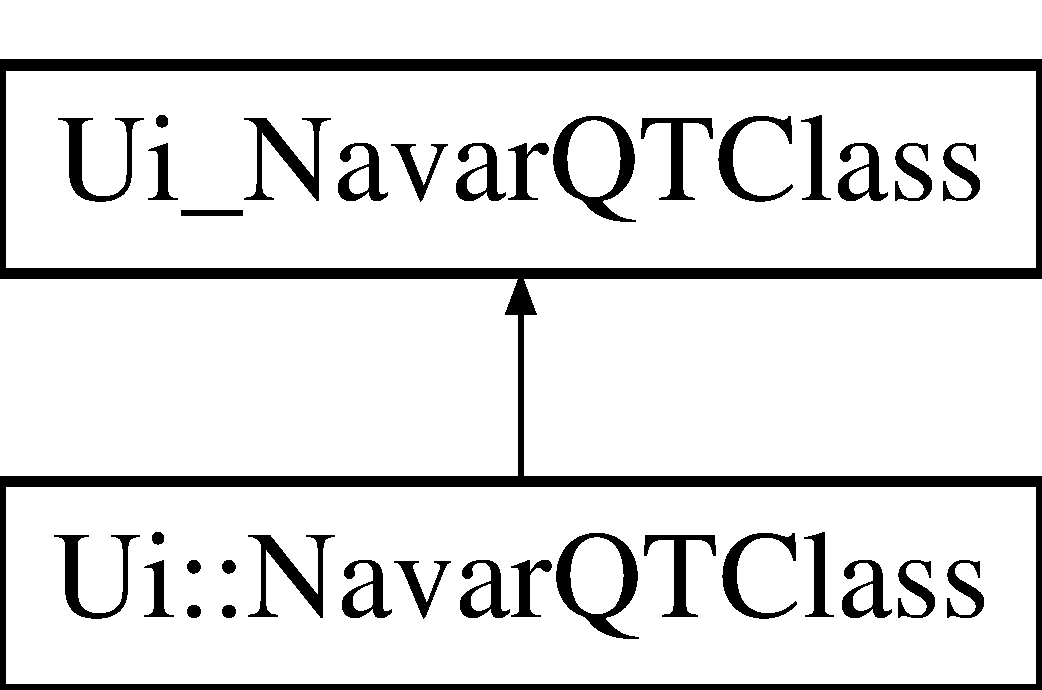
\includegraphics[height=2.000000cm]{class_ui_1_1_navar_q_t_class}
\end{center}
\end{figure}
\subsection*{Additional Inherited Members}


The documentation for this class was generated from the following file\+:\begin{DoxyCompactItemize}
\item 
C\+:/\+Users/eduar\+\_\+000/\+Documents/\+Visual Studio 2015/\+Projects/\+Navar\+Q\+A/\+Navar\+Q\+A/\+Generated\+Files/ui\+\_\+\+Navar\+Q\+T.\+h\end{DoxyCompactItemize}

\hypertarget{struct_custom_camera_library_1_1_output}{}\section{Custom\+Camera\+Library\+:\+:Output Struct Reference}
\label{struct_custom_camera_library_1_1_output}\index{Custom\+Camera\+Library\+::\+Output@{Custom\+Camera\+Library\+::\+Output}}


Esta estructura permite almacenar las características de los cuerpos rígidos que vayan siendo detectados en mientras se esta ejecutando la la función Custom\+Camera\+Library\+::joskstra()  




{\ttfamily \#include $<$detectbr.\+h$>$}

\subsection*{Public Attributes}
\begin{DoxyCompactItemize}
\item 
int \hyperlink{struct_custom_camera_library_1_1_output_a035a9b6775bc3cd9637f8b67018f628b}{bdr}
\item 
string \hyperlink{struct_custom_camera_library_1_1_output_af0a8276215ad6447ca0391d32ffe72f5}{name}
\item 
Mat\+\_\+$<$ double $>$ \hyperlink{struct_custom_camera_library_1_1_output_ae2017d51295ddb45390dc715b4815b29}{bdrigid}
\item 
Mat\+\_\+$<$ double $>$ \hyperlink{struct_custom_camera_library_1_1_output_a06fa54e7fbbd5075e6517b9a6c93ca97}{centroid}
\item 
int \hyperlink{struct_custom_camera_library_1_1_output_a3361db4b0b8107c1458feebbb50c0589}{nmarkers}
\item 
double \hyperlink{struct_custom_camera_library_1_1_output_a7fa444f6b387695a1b29c460fe5f1bad}{yaw}
\item 
double \hyperlink{struct_custom_camera_library_1_1_output_a2ecfe8192c7cc66e5d3385c21ef4ab39}{pitch}
\item 
double \hyperlink{struct_custom_camera_library_1_1_output_a9383b78c1f441b6c816533c0011c2478}{roll}
\item 
Point3d \hyperlink{struct_custom_camera_library_1_1_output_aa8d02d07cd889dd98ed76942616cd06c}{point}
\item 
Mat\+\_\+$<$ double $>$ \hyperlink{struct_custom_camera_library_1_1_output_a5fab2e3e26e7e4ebb82046f2c28899a7}{Quat}
\end{DoxyCompactItemize}


\subsection{Detailed Description}
Esta estructura permite almacenar las características de los cuerpos rígidos que vayan siendo detectados en mientras se esta ejecutando la la función Custom\+Camera\+Library\+::joskstra() 

\subsection{Member Data Documentation}
\index{Custom\+Camera\+Library\+::\+Output@{Custom\+Camera\+Library\+::\+Output}!bdr@{bdr}}
\index{bdr@{bdr}!Custom\+Camera\+Library\+::\+Output@{Custom\+Camera\+Library\+::\+Output}}
\subsubsection[{\texorpdfstring{bdr}{bdr}}]{\setlength{\rightskip}{0pt plus 5cm}Custom\+Camera\+Library\+::\+Output\+::bdr}\hypertarget{struct_custom_camera_library_1_1_output_a035a9b6775bc3cd9637f8b67018f628b}{}\label{struct_custom_camera_library_1_1_output_a035a9b6775bc3cd9637f8b67018f628b}
Contiene el número que identifica un cuerpo rígido, los números que identifican a un cuerpo rígido son\+:
\begin{DoxyItemize}
\item Pointer = 1
\item Femur = 2
\item Tíbia = 3
\item Gafas = 4

Este orden es obtenido de la matriz de distancias de cuerpos rígidos. \begin{DoxySeeAlso}{See also}
Custom\+Camera\+Library\+::distances 
\end{DoxySeeAlso}

\end{DoxyItemize}\index{Custom\+Camera\+Library\+::\+Output@{Custom\+Camera\+Library\+::\+Output}!bdrigid@{bdrigid}}
\index{bdrigid@{bdrigid}!Custom\+Camera\+Library\+::\+Output@{Custom\+Camera\+Library\+::\+Output}}
\subsubsection[{\texorpdfstring{bdrigid}{bdrigid}}]{\setlength{\rightskip}{0pt plus 5cm}Custom\+Camera\+Library\+::\+Output\+::bdrigid}\hypertarget{struct_custom_camera_library_1_1_output_ae2017d51295ddb45390dc715b4815b29}{}\label{struct_custom_camera_library_1_1_output_ae2017d51295ddb45390dc715b4815b29}
Matriz que contiene las coordenadas {\itshape x}, {\itshape y}, {\itshape z} de un cuerpo rígido detectado. \index{Custom\+Camera\+Library\+::\+Output@{Custom\+Camera\+Library\+::\+Output}!centroid@{centroid}}
\index{centroid@{centroid}!Custom\+Camera\+Library\+::\+Output@{Custom\+Camera\+Library\+::\+Output}}
\subsubsection[{\texorpdfstring{centroid}{centroid}}]{\setlength{\rightskip}{0pt plus 5cm}Custom\+Camera\+Library\+::\+Output\+::centroid}\hypertarget{struct_custom_camera_library_1_1_output_a06fa54e7fbbd5075e6517b9a6c93ca97}{}\label{struct_custom_camera_library_1_1_output_a06fa54e7fbbd5075e6517b9a6c93ca97}
Matriz 3x1 que contiene la coordenada del centro del circulo que forma los marcadores que componen el cuerpo rígido. \index{Custom\+Camera\+Library\+::\+Output@{Custom\+Camera\+Library\+::\+Output}!name@{name}}
\index{name@{name}!Custom\+Camera\+Library\+::\+Output@{Custom\+Camera\+Library\+::\+Output}}
\subsubsection[{\texorpdfstring{name}{name}}]{\setlength{\rightskip}{0pt plus 5cm}Custom\+Camera\+Library\+::\+Output\+::name}\hypertarget{struct_custom_camera_library_1_1_output_af0a8276215ad6447ca0391d32ffe72f5}{}\label{struct_custom_camera_library_1_1_output_af0a8276215ad6447ca0391d32ffe72f5}
Nombre del objeto rígido (F\+E\+M\+UR, P\+O\+I\+N\+T\+ER, T\+I\+B\+IA, G\+A\+F\+AS). \index{Custom\+Camera\+Library\+::\+Output@{Custom\+Camera\+Library\+::\+Output}!nmarkers@{nmarkers}}
\index{nmarkers@{nmarkers}!Custom\+Camera\+Library\+::\+Output@{Custom\+Camera\+Library\+::\+Output}}
\subsubsection[{\texorpdfstring{nmarkers}{nmarkers}}]{\setlength{\rightskip}{0pt plus 5cm}Custom\+Camera\+Library\+::\+Output\+::nmarkers}\hypertarget{struct_custom_camera_library_1_1_output_a3361db4b0b8107c1458feebbb50c0589}{}\label{struct_custom_camera_library_1_1_output_a3361db4b0b8107c1458feebbb50c0589}
Número de marcadores que forman el cuerpo rígido. \index{Custom\+Camera\+Library\+::\+Output@{Custom\+Camera\+Library\+::\+Output}!pitch@{pitch}}
\index{pitch@{pitch}!Custom\+Camera\+Library\+::\+Output@{Custom\+Camera\+Library\+::\+Output}}
\subsubsection[{\texorpdfstring{pitch}{pitch}}]{\setlength{\rightskip}{0pt plus 5cm}Custom\+Camera\+Library\+::\+Output\+::pitch}\hypertarget{struct_custom_camera_library_1_1_output_a2ecfe8192c7cc66e5d3385c21ef4ab39}{}\label{struct_custom_camera_library_1_1_output_a2ecfe8192c7cc66e5d3385c21ef4ab39}
Ángulo de euler en grados. \index{Custom\+Camera\+Library\+::\+Output@{Custom\+Camera\+Library\+::\+Output}!point@{point}}
\index{point@{point}!Custom\+Camera\+Library\+::\+Output@{Custom\+Camera\+Library\+::\+Output}}
\subsubsection[{\texorpdfstring{point}{point}}]{\setlength{\rightskip}{0pt plus 5cm}Custom\+Camera\+Library\+::\+Output\+::point}\hypertarget{struct_custom_camera_library_1_1_output_aa8d02d07cd889dd98ed76942616cd06c}{}\label{struct_custom_camera_library_1_1_output_aa8d02d07cd889dd98ed76942616cd06c}
Si el objeto rígido detectado es el pointer entonces esta propiedad tendrá el valor del punto que toca la punta, de lo contrario será nulo el valor. \index{Custom\+Camera\+Library\+::\+Output@{Custom\+Camera\+Library\+::\+Output}!Quat@{Quat}}
\index{Quat@{Quat}!Custom\+Camera\+Library\+::\+Output@{Custom\+Camera\+Library\+::\+Output}}
\subsubsection[{\texorpdfstring{Quat}{Quat}}]{\setlength{\rightskip}{0pt plus 5cm}Custom\+Camera\+Library\+::\+Output\+::\+Quat}\hypertarget{struct_custom_camera_library_1_1_output_a5fab2e3e26e7e4ebb82046f2c28899a7}{}\label{struct_custom_camera_library_1_1_output_a5fab2e3e26e7e4ebb82046f2c28899a7}
Cuaternios que representan la orientación del objeto rígido. \index{Custom\+Camera\+Library\+::\+Output@{Custom\+Camera\+Library\+::\+Output}!roll@{roll}}
\index{roll@{roll}!Custom\+Camera\+Library\+::\+Output@{Custom\+Camera\+Library\+::\+Output}}
\subsubsection[{\texorpdfstring{roll}{roll}}]{\setlength{\rightskip}{0pt plus 5cm}Custom\+Camera\+Library\+::\+Output\+::roll}\hypertarget{struct_custom_camera_library_1_1_output_a9383b78c1f441b6c816533c0011c2478}{}\label{struct_custom_camera_library_1_1_output_a9383b78c1f441b6c816533c0011c2478}
Ángulo de euler en grados. \index{Custom\+Camera\+Library\+::\+Output@{Custom\+Camera\+Library\+::\+Output}!yaw@{yaw}}
\index{yaw@{yaw}!Custom\+Camera\+Library\+::\+Output@{Custom\+Camera\+Library\+::\+Output}}
\subsubsection[{\texorpdfstring{yaw}{yaw}}]{\setlength{\rightskip}{0pt plus 5cm}Custom\+Camera\+Library\+::\+Output\+::yaw}\hypertarget{struct_custom_camera_library_1_1_output_a7fa444f6b387695a1b29c460fe5f1bad}{}\label{struct_custom_camera_library_1_1_output_a7fa444f6b387695a1b29c460fe5f1bad}
Ángulo de euler en grados. 

The documentation for this struct was generated from the following file\+:\begin{DoxyCompactItemize}
\item 
C\+:/\+Users/eduar\+\_\+000/\+Documents/\+Visual Studio 2015/\+Projects/\+Navar\+Q\+A/\+Navar\+Q\+A/detectbr.\+h\end{DoxyCompactItemize}

\hypertarget{classpointer_calib}{}\section{pointer\+Calib Class Reference}
\label{classpointer_calib}\index{pointer\+Calib@{pointer\+Calib}}
\subsection*{Public Member Functions}
\begin{DoxyCompactItemize}
\item 
void {\bfseries update\+Cordinates} (cv\+::\+Mat\+\_\+$<$ double $>$ \&origin)\hypertarget{classpointer_calib_a3146722337ba0faab6d61ddb4f662aa6}{}\label{classpointer_calib_a3146722337ba0faab6d61ddb4f662aa6}

\end{DoxyCompactItemize}


The documentation for this class was generated from the following files\+:\begin{DoxyCompactItemize}
\item 
C\+:/\+Users/eduar\+\_\+000/\+Documents/\+Visual Studio 2015/\+Projects/\+Navar\+Q\+A/\+Navar\+Q\+A/pointer\+Calib.\+h\item 
C\+:/\+Users/eduar\+\_\+000/\+Documents/\+Visual Studio 2015/\+Projects/\+Navar\+Q\+A/\+Navar\+Q\+A/pointer\+Calib.\+cpp\end{DoxyCompactItemize}

\hypertarget{structqt__meta__stringdata___g_u_i_updater__t}{}\section{qt\+\_\+meta\+\_\+stringdata\+\_\+\+G\+U\+I\+Updater\+\_\+t Struct Reference}
\label{structqt__meta__stringdata___g_u_i_updater__t}\index{qt\+\_\+meta\+\_\+stringdata\+\_\+\+G\+U\+I\+Updater\+\_\+t@{qt\+\_\+meta\+\_\+stringdata\+\_\+\+G\+U\+I\+Updater\+\_\+t}}
\subsection*{Public Attributes}
\begin{DoxyCompactItemize}
\item 
Q\+Byte\+Array\+Data {\bfseries data} \mbox{[}9\mbox{]}\hypertarget{structqt__meta__stringdata___g_u_i_updater__t_ad7ffa7f7e40232a6072953c340083c7c}{}\label{structqt__meta__stringdata___g_u_i_updater__t_ad7ffa7f7e40232a6072953c340083c7c}

\item 
char {\bfseries stringdata0} \mbox{[}119\mbox{]}\hypertarget{structqt__meta__stringdata___g_u_i_updater__t_ae431608bb6b8a869877e165c0d85e8ba}{}\label{structqt__meta__stringdata___g_u_i_updater__t_ae431608bb6b8a869877e165c0d85e8ba}

\end{DoxyCompactItemize}


The documentation for this struct was generated from the following file\+:\begin{DoxyCompactItemize}
\item 
C\+:/\+Users/eduar\+\_\+000/\+Documents/\+Visual Studio 2015/\+Projects/\+Navar\+Q\+A/\+Navar\+Q\+A/\+Generated\+Files/\+Debug/moc\+\_\+\+G\+U\+I\+Updater.\+cpp\end{DoxyCompactItemize}

\hypertarget{structqt__meta__stringdata___navar_q_t__t}{}\section{qt\+\_\+meta\+\_\+stringdata\+\_\+\+Navar\+Q\+T\+\_\+t Struct Reference}
\label{structqt__meta__stringdata___navar_q_t__t}\index{qt\+\_\+meta\+\_\+stringdata\+\_\+\+Navar\+Q\+T\+\_\+t@{qt\+\_\+meta\+\_\+stringdata\+\_\+\+Navar\+Q\+T\+\_\+t}}
\subsection*{Public Attributes}
\begin{DoxyCompactItemize}
\item 
Q\+Byte\+Array\+Data {\bfseries data} \mbox{[}27\mbox{]}\hypertarget{structqt__meta__stringdata___navar_q_t__t_a064fea1a0caa2cef65cc1c84352fada2}{}\label{structqt__meta__stringdata___navar_q_t__t_a064fea1a0caa2cef65cc1c84352fada2}

\item 
char {\bfseries stringdata0} \mbox{[}560\mbox{]}\hypertarget{structqt__meta__stringdata___navar_q_t__t_ad8e2a9ea1719500771c4be791ff0fa3c}{}\label{structqt__meta__stringdata___navar_q_t__t_ad8e2a9ea1719500771c4be791ff0fa3c}

\end{DoxyCompactItemize}


The documentation for this struct was generated from the following file\+:\begin{DoxyCompactItemize}
\item 
C\+:/\+Users/eduar\+\_\+000/\+Documents/\+Visual Studio 2015/\+Projects/\+Navar\+Q\+A/\+Navar\+Q\+A/\+Generated\+Files/\+Debug/moc\+\_\+\+Navar\+Q\+T.\+cpp\end{DoxyCompactItemize}

\hypertarget{struct_quat}{}\section{Quat Struct Reference}
\label{struct_quat}\index{Quat@{Quat}}
\subsection*{Public Attributes}
\begin{DoxyCompactItemize}
\item 
float {\bfseries x}\hypertarget{struct_quat_a15db053bd6750a53e33bf30a0250c288}{}\label{struct_quat_a15db053bd6750a53e33bf30a0250c288}

\item 
float {\bfseries y}\hypertarget{struct_quat_ac6045ee4149a978a4ce429c132e46fa2}{}\label{struct_quat_ac6045ee4149a978a4ce429c132e46fa2}

\item 
float {\bfseries z}\hypertarget{struct_quat_a611fbb79f7b802da4f1c65a31c2c5fea}{}\label{struct_quat_a611fbb79f7b802da4f1c65a31c2c5fea}

\item 
float {\bfseries w}\hypertarget{struct_quat_ad3aeee2134443ec0897793834209b0c0}{}\label{struct_quat_ad3aeee2134443ec0897793834209b0c0}

\end{DoxyCompactItemize}


The documentation for this struct was generated from the following file\+:\begin{DoxyCompactItemize}
\item 
C\+:/\+Users/eduar\+\_\+000/\+Documents/\+Visual Studio 2015/\+Projects/\+Navar\+Q\+A/\+Navar\+Q\+A/N\+A\+T\+Utils.\+h\end{DoxyCompactItemize}

\hypertarget{class_ui___navar_q_t_class}{}\section{Ui\+\_\+\+Navar\+Q\+T\+Class Class Reference}
\label{class_ui___navar_q_t_class}\index{Ui\+\_\+\+Navar\+Q\+T\+Class@{Ui\+\_\+\+Navar\+Q\+T\+Class}}
Inheritance diagram for Ui\+\_\+\+Navar\+Q\+T\+Class\+:\begin{figure}[H]
\begin{center}
\leavevmode
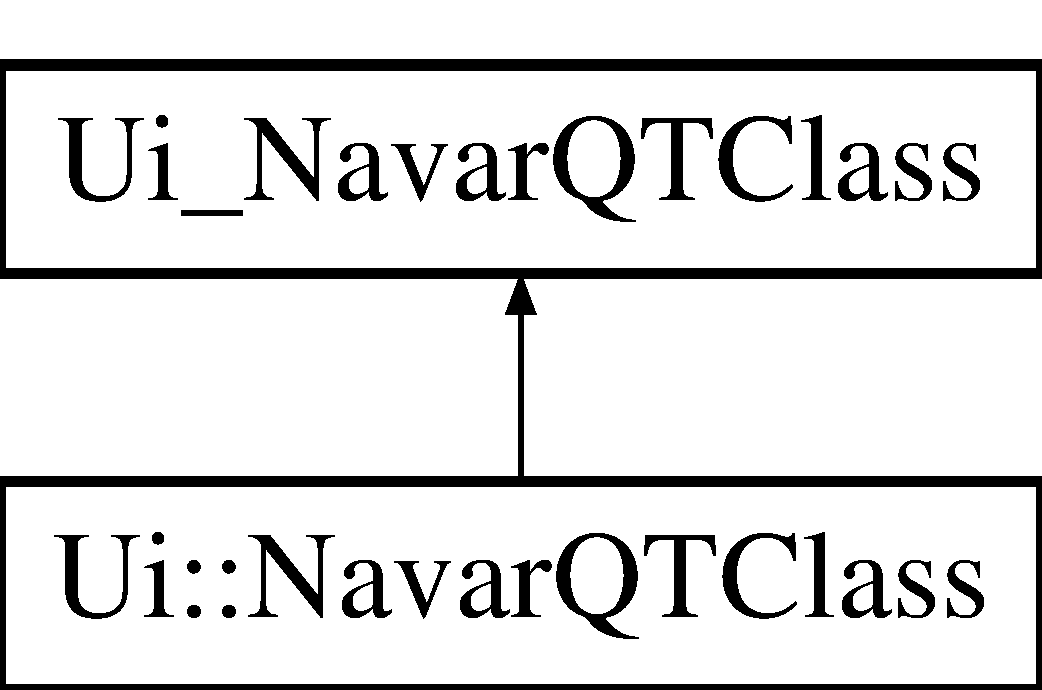
\includegraphics[height=2.000000cm]{class_ui___navar_q_t_class}
\end{center}
\end{figure}
\subsection*{Public Member Functions}
\begin{DoxyCompactItemize}
\item 
void {\bfseries setup\+Ui} (Q\+Widget $\ast$Navar\+Q\+T\+Class)\hypertarget{class_ui___navar_q_t_class_af668d39ae0db534cc6f2e421fe2b4d8c}{}\label{class_ui___navar_q_t_class_af668d39ae0db534cc6f2e421fe2b4d8c}

\item 
void {\bfseries retranslate\+Ui} (Q\+Widget $\ast$Navar\+Q\+T\+Class)\hypertarget{class_ui___navar_q_t_class_a610b6553965ebad6e4accddcebe39a7f}{}\label{class_ui___navar_q_t_class_a610b6553965ebad6e4accddcebe39a7f}

\end{DoxyCompactItemize}
\subsection*{Public Attributes}
\begin{DoxyCompactItemize}
\item 
Q\+Grid\+Layout $\ast$ {\bfseries grid\+Layout}\hypertarget{class_ui___navar_q_t_class_ac917b56bee44b4f2dcbcea7c9b870a1e}{}\label{class_ui___navar_q_t_class_ac917b56bee44b4f2dcbcea7c9b870a1e}

\item 
Q\+Widget $\ast$ {\bfseries header}\hypertarget{class_ui___navar_q_t_class_aa70fb543a044c18cc933ad44e91eb3d1}{}\label{class_ui___navar_q_t_class_aa70fb543a044c18cc933ad44e91eb3d1}

\item 
Q\+Grid\+Layout $\ast$ {\bfseries grid\+Layout\+\_\+11}\hypertarget{class_ui___navar_q_t_class_a4e3846b2a2765c4473d084a273885a0d}{}\label{class_ui___navar_q_t_class_a4e3846b2a2765c4473d084a273885a0d}

\item 
Q\+Push\+Button $\ast$ {\bfseries push\+Button\+\_\+close}\hypertarget{class_ui___navar_q_t_class_a4fb956f52699ecde743c460bb7cbad85}{}\label{class_ui___navar_q_t_class_a4fb956f52699ecde743c460bb7cbad85}

\item 
Q\+Spacer\+Item $\ast$ {\bfseries horizontal\+Spacer\+\_\+3}\hypertarget{class_ui___navar_q_t_class_a82b1a287b77babbed5bf34fcb0c59de2}{}\label{class_ui___navar_q_t_class_a82b1a287b77babbed5bf34fcb0c59de2}

\item 
Q\+Widget $\ast$ {\bfseries steps}\hypertarget{class_ui___navar_q_t_class_ad89479d3173a7f10b7cbb6aa6f58a06b}{}\label{class_ui___navar_q_t_class_ad89479d3173a7f10b7cbb6aa6f58a06b}

\item 
Q\+Grid\+Layout $\ast$ {\bfseries grid\+Layout\+\_\+3}\hypertarget{class_ui___navar_q_t_class_a63936277b77492ee8892019961c7f407}{}\label{class_ui___navar_q_t_class_a63936277b77492ee8892019961c7f407}

\item 
Q\+Push\+Button $\ast$ {\bfseries push\+Button\+\_\+step\+\_\+2}\hypertarget{class_ui___navar_q_t_class_a084cfe909f021bbb02f5bb6d510b0d7c}{}\label{class_ui___navar_q_t_class_a084cfe909f021bbb02f5bb6d510b0d7c}

\item 
Q\+Push\+Button $\ast$ {\bfseries push\+Button\+\_\+step\+\_\+1}\hypertarget{class_ui___navar_q_t_class_aaef76d2aa833be3664d30d6dc565f637}{}\label{class_ui___navar_q_t_class_aaef76d2aa833be3664d30d6dc565f637}

\item 
Q\+Push\+Button $\ast$ {\bfseries push\+Button\+\_\+step\+\_\+4}\hypertarget{class_ui___navar_q_t_class_a1344352f453b450fd4f9aa89cccfbf97}{}\label{class_ui___navar_q_t_class_a1344352f453b450fd4f9aa89cccfbf97}

\item 
Q\+Push\+Button $\ast$ {\bfseries push\+Button\+\_\+step\+\_\+3}\hypertarget{class_ui___navar_q_t_class_aba401ed637811db08de5c11f2b0ba0ae}{}\label{class_ui___navar_q_t_class_aba401ed637811db08de5c11f2b0ba0ae}

\item 
Q\+Stacked\+Widget $\ast$ {\bfseries body}\hypertarget{class_ui___navar_q_t_class_a990aba8d1635cb750c26a63926cce11c}{}\label{class_ui___navar_q_t_class_a990aba8d1635cb750c26a63926cce11c}

\item 
Q\+Widget $\ast$ {\bfseries setup\+\_\+page}\hypertarget{class_ui___navar_q_t_class_a3d66259ece36fd09675c808da35e7704}{}\label{class_ui___navar_q_t_class_a3d66259ece36fd09675c808da35e7704}

\item 
Q\+Grid\+Layout $\ast$ {\bfseries grid\+Layout\+\_\+2}\hypertarget{class_ui___navar_q_t_class_af40e813392ba4c9148a977f8aa5a6930}{}\label{class_ui___navar_q_t_class_af40e813392ba4c9148a977f8aa5a6930}

\item 
Q\+Label $\ast$ {\bfseries label\+\_\+camera\+\_\+left}\hypertarget{class_ui___navar_q_t_class_ab9133803f7d005cf0cd4909228101831}{}\label{class_ui___navar_q_t_class_ab9133803f7d005cf0cd4909228101831}

\item 
Q\+Label $\ast$ {\bfseries label\+\_\+camera\+\_\+right}\hypertarget{class_ui___navar_q_t_class_a9cbd1075e1fe2572d9b3f20122f3d8d6}{}\label{class_ui___navar_q_t_class_a9cbd1075e1fe2572d9b3f20122f3d8d6}

\item 
Q\+Widget $\ast$ {\bfseries instructions}\hypertarget{class_ui___navar_q_t_class_ab3fe914ee2120e61f84872b99004df58}{}\label{class_ui___navar_q_t_class_ab3fe914ee2120e61f84872b99004df58}

\item 
Q\+V\+Box\+Layout $\ast$ {\bfseries vertical\+Layout}\hypertarget{class_ui___navar_q_t_class_a2f3061117d3a7ac9c8365d7472cd65fc}{}\label{class_ui___navar_q_t_class_a2f3061117d3a7ac9c8365d7472cd65fc}

\item 
Q\+Push\+Button $\ast$ {\bfseries push\+Button\+\_\+4}\hypertarget{class_ui___navar_q_t_class_ab97415e1dc3841208a9e8071cf0a1e65}{}\label{class_ui___navar_q_t_class_ab97415e1dc3841208a9e8071cf0a1e65}

\item 
Q\+Push\+Button $\ast$ {\bfseries push\+Button\+\_\+5}\hypertarget{class_ui___navar_q_t_class_a3db5fc479881cb7471e98cc6eaf252a8}{}\label{class_ui___navar_q_t_class_a3db5fc479881cb7471e98cc6eaf252a8}

\item 
Q\+Push\+Button $\ast$ {\bfseries push\+Button\+\_\+6}\hypertarget{class_ui___navar_q_t_class_a523ce098d0543e0a786d1324811cd324}{}\label{class_ui___navar_q_t_class_a523ce098d0543e0a786d1324811cd324}

\item 
Q\+Push\+Button $\ast$ {\bfseries push\+Button\+\_\+7}\hypertarget{class_ui___navar_q_t_class_a7347d0da046f1e5210a1505e5418a7bf}{}\label{class_ui___navar_q_t_class_a7347d0da046f1e5210a1505e5418a7bf}

\item 
Q\+Push\+Button $\ast$ {\bfseries push\+Button\+\_\+8}\hypertarget{class_ui___navar_q_t_class_a7d83bdebcaae437efef8547b21f28358}{}\label{class_ui___navar_q_t_class_a7d83bdebcaae437efef8547b21f28358}

\item 
Q\+Widget $\ast$ {\bfseries controls}\hypertarget{class_ui___navar_q_t_class_a8b90ccc72f680cc20c8150a9222ebd38}{}\label{class_ui___navar_q_t_class_a8b90ccc72f680cc20c8150a9222ebd38}

\item 
Q\+V\+Box\+Layout $\ast$ {\bfseries vertical\+Layout\+\_\+2}\hypertarget{class_ui___navar_q_t_class_a8e8a41869aeced4a370332cf5e21b118}{}\label{class_ui___navar_q_t_class_a8e8a41869aeced4a370332cf5e21b118}

\item 
Q\+Combo\+Box $\ast$ {\bfseries combo\+Box}\hypertarget{class_ui___navar_q_t_class_a12b0329ed308a1f97abf1cc26b55a1e2}{}\label{class_ui___navar_q_t_class_a12b0329ed308a1f97abf1cc26b55a1e2}

\item 
Q\+Label $\ast$ {\bfseries label\+\_\+6}\hypertarget{class_ui___navar_q_t_class_aba5cb17a57a18a3cf97a427913dec1a3}{}\label{class_ui___navar_q_t_class_aba5cb17a57a18a3cf97a427913dec1a3}

\item 
Q\+Push\+Button $\ast$ {\bfseries push\+Button\+\_\+3}\hypertarget{class_ui___navar_q_t_class_a62744350788cb622e6a0a9c467f8fb9f}{}\label{class_ui___navar_q_t_class_a62744350788cb622e6a0a9c467f8fb9f}

\item 
Q\+Push\+Button $\ast$ {\bfseries push\+Button\+\_\+10}\hypertarget{class_ui___navar_q_t_class_a4eae6a4b2d27f9c99e17ceb4f0bb9aac}{}\label{class_ui___navar_q_t_class_a4eae6a4b2d27f9c99e17ceb4f0bb9aac}

\item 
Q\+Label $\ast$ {\bfseries label\+\_\+instructions\+\_\+bottom}\hypertarget{class_ui___navar_q_t_class_a86f339656a3658639d6d6d91cdbb54d8}{}\label{class_ui___navar_q_t_class_a86f339656a3658639d6d6d91cdbb54d8}

\item 
Q\+Widget $\ast$ {\bfseries login\+\_\+page}\hypertarget{class_ui___navar_q_t_class_afd04ad703a1dbf6cce6808f3d9516f2b}{}\label{class_ui___navar_q_t_class_afd04ad703a1dbf6cce6808f3d9516f2b}

\item 
Q\+Grid\+Layout $\ast$ {\bfseries grid\+Layout\+\_\+5}\hypertarget{class_ui___navar_q_t_class_aaf7eee5bee6534570d51b4149021cf2c}{}\label{class_ui___navar_q_t_class_aaf7eee5bee6534570d51b4149021cf2c}

\item 
Q\+Group\+Box $\ast$ {\bfseries group\+Box}\hypertarget{class_ui___navar_q_t_class_abbf020fd7a3941fdca527ae14fc83b3b}{}\label{class_ui___navar_q_t_class_abbf020fd7a3941fdca527ae14fc83b3b}

\item 
Q\+Grid\+Layout $\ast$ {\bfseries grid\+Layout\+\_\+4}\hypertarget{class_ui___navar_q_t_class_a21a2d137cf26900f3d494f82c54e2326}{}\label{class_ui___navar_q_t_class_a21a2d137cf26900f3d494f82c54e2326}

\item 
Q\+Label $\ast$ {\bfseries label\+\_\+login\+\_\+image}\hypertarget{class_ui___navar_q_t_class_aeb3ef969709e75f11f439f662dbd839b}{}\label{class_ui___navar_q_t_class_aeb3ef969709e75f11f439f662dbd839b}

\item 
Q\+Line\+Edit $\ast$ {\bfseries line\+Edit\+\_\+user}\hypertarget{class_ui___navar_q_t_class_a662e6bbe7cc4cb10c21a2ab2512866f4}{}\label{class_ui___navar_q_t_class_a662e6bbe7cc4cb10c21a2ab2512866f4}

\item 
Q\+Push\+Button $\ast$ {\bfseries push\+Button\+\_\+1}\hypertarget{class_ui___navar_q_t_class_ab312b63867c13737d28d2ace36e79de7}{}\label{class_ui___navar_q_t_class_ab312b63867c13737d28d2ace36e79de7}

\item 
Q\+Line\+Edit $\ast$ {\bfseries line\+Edit\+\_\+password}\hypertarget{class_ui___navar_q_t_class_af5df09cfcd306cbdbdd440fc409955a8}{}\label{class_ui___navar_q_t_class_af5df09cfcd306cbdbdd440fc409955a8}

\item 
Q\+Spacer\+Item $\ast$ {\bfseries vertical\+Spacer}\hypertarget{class_ui___navar_q_t_class_acbaca83c7d11792b63edc4685d242df1}{}\label{class_ui___navar_q_t_class_acbaca83c7d11792b63edc4685d242df1}

\item 
Q\+Spacer\+Item $\ast$ {\bfseries horizontal\+Spacer}\hypertarget{class_ui___navar_q_t_class_ade4ffd6f288bd7491b0d1a0cfa8d652d}{}\label{class_ui___navar_q_t_class_ade4ffd6f288bd7491b0d1a0cfa8d652d}

\item 
Q\+Spacer\+Item $\ast$ {\bfseries horizontal\+Spacer\+\_\+2}\hypertarget{class_ui___navar_q_t_class_a1055db9d96d92eb4e89588effffec49f}{}\label{class_ui___navar_q_t_class_a1055db9d96d92eb4e89588effffec49f}

\item 
Q\+Spacer\+Item $\ast$ {\bfseries vertical\+Spacer\+\_\+2}\hypertarget{class_ui___navar_q_t_class_a984f6216e8be4a84bdf0923609adc7c2}{}\label{class_ui___navar_q_t_class_a984f6216e8be4a84bdf0923609adc7c2}

\item 
Q\+Widget $\ast$ {\bfseries surgery\+\_\+page}\hypertarget{class_ui___navar_q_t_class_a7d46a8ebed1d940d229cba2acab30a40}{}\label{class_ui___navar_q_t_class_a7d46a8ebed1d940d229cba2acab30a40}

\item 
Q\+Grid\+Layout $\ast$ {\bfseries grid\+Layout\+\_\+9}\hypertarget{class_ui___navar_q_t_class_ad346db6c224ac29dcb30de54076d754f}{}\label{class_ui___navar_q_t_class_ad346db6c224ac29dcb30de54076d754f}

\item 
Q\+Scroll\+Area $\ast$ {\bfseries scroll\+Area\+\_\+cases}\hypertarget{class_ui___navar_q_t_class_a2db6c6470bb66ddfbbbb3cd9ba1364af}{}\label{class_ui___navar_q_t_class_a2db6c6470bb66ddfbbbb3cd9ba1364af}

\item 
Q\+Widget $\ast$ {\bfseries scroll\+Area\+Widget\+Contents}\hypertarget{class_ui___navar_q_t_class_a179ac37690c7d23f2a624b492ef67051}{}\label{class_ui___navar_q_t_class_a179ac37690c7d23f2a624b492ef67051}

\item 
Q\+Grid\+Layout $\ast$ {\bfseries grid\+Layout\+\_\+7}\hypertarget{class_ui___navar_q_t_class_a52da6c0d06bcce719d79ae5381d8c9cd}{}\label{class_ui___navar_q_t_class_a52da6c0d06bcce719d79ae5381d8c9cd}

\item 
Q\+Widget $\ast$ {\bfseries widget\+\_\+2}\hypertarget{class_ui___navar_q_t_class_ade8af222f2f8c4a951be1209dff1004d}{}\label{class_ui___navar_q_t_class_ade8af222f2f8c4a951be1209dff1004d}

\item 
Q\+Grid\+Layout $\ast$ {\bfseries grid\+Layout\+\_\+6}\hypertarget{class_ui___navar_q_t_class_ac9865aca386379a2ac272a1498c4bce3}{}\label{class_ui___navar_q_t_class_ac9865aca386379a2ac272a1498c4bce3}

\item 
Q\+Label $\ast$ {\bfseries label\+\_\+2}\hypertarget{class_ui___navar_q_t_class_a5b4b808fac1237c1a7c63dd62462efd5}{}\label{class_ui___navar_q_t_class_a5b4b808fac1237c1a7c63dd62462efd5}

\item 
Q\+Label $\ast$ {\bfseries label\+\_\+3}\hypertarget{class_ui___navar_q_t_class_a24af6f649b97171b04527e7d24f01877}{}\label{class_ui___navar_q_t_class_a24af6f649b97171b04527e7d24f01877}

\item 
Q\+Push\+Button $\ast$ {\bfseries push\+Button\+\_\+case\+\_\+11}\hypertarget{class_ui___navar_q_t_class_af4af9c58a12429037c492fb1a7398e0a}{}\label{class_ui___navar_q_t_class_af4af9c58a12429037c492fb1a7398e0a}

\item 
Q\+Push\+Button $\ast$ {\bfseries push\+Button\+\_\+case\+\_\+12}\hypertarget{class_ui___navar_q_t_class_a21cb0c37b9e27d2acc7cba8625586283}{}\label{class_ui___navar_q_t_class_a21cb0c37b9e27d2acc7cba8625586283}

\item 
Q\+Push\+Button $\ast$ {\bfseries push\+Button\+\_\+case\+\_\+13}\hypertarget{class_ui___navar_q_t_class_a871efa91af431bfc4e992e99c241fc6f}{}\label{class_ui___navar_q_t_class_a871efa91af431bfc4e992e99c241fc6f}

\item 
Q\+Label $\ast$ {\bfseries label\+\_\+case\+\_\+title}\hypertarget{class_ui___navar_q_t_class_a833279da705c73e6303958707fa9acec}{}\label{class_ui___navar_q_t_class_a833279da705c73e6303958707fa9acec}

\item 
Q\+Spacer\+Item $\ast$ {\bfseries vertical\+Spacer\+\_\+3}\hypertarget{class_ui___navar_q_t_class_af410a14c6560f45ea5122fa0b5c55233}{}\label{class_ui___navar_q_t_class_af410a14c6560f45ea5122fa0b5c55233}

\item 
Q\+Widget $\ast$ {\bfseries widget\+\_\+cases\+\_\+view}\hypertarget{class_ui___navar_q_t_class_a803c4dd26abdd107e76b819ce76d5b4b}{}\label{class_ui___navar_q_t_class_a803c4dd26abdd107e76b819ce76d5b4b}

\item 
Q\+Grid\+Layout $\ast$ {\bfseries grid\+Layout\+\_\+8}\hypertarget{class_ui___navar_q_t_class_a9d9d46f0bed9ebb060686f96082258a7}{}\label{class_ui___navar_q_t_class_a9d9d46f0bed9ebb060686f96082258a7}

\item 
Q\+Label $\ast$ {\bfseries label}\hypertarget{class_ui___navar_q_t_class_a37aa500487454ae5811c71d1cc41ac5b}{}\label{class_ui___navar_q_t_class_a37aa500487454ae5811c71d1cc41ac5b}

\item 
Q\+Label $\ast$ {\bfseries label\+\_\+4}\hypertarget{class_ui___navar_q_t_class_a34f81b01eda90da73238859a0efe2911}{}\label{class_ui___navar_q_t_class_a34f81b01eda90da73238859a0efe2911}

\item 
Q\+Tab\+Widget $\ast$ {\bfseries tab\+Widget\+\_\+cases\+\_\+view}\hypertarget{class_ui___navar_q_t_class_a5e16329bea8e825d0e3427ac64fef21d}{}\label{class_ui___navar_q_t_class_a5e16329bea8e825d0e3427ac64fef21d}

\item 
Q\+Widget $\ast$ {\bfseries tab\+\_\+1}\hypertarget{class_ui___navar_q_t_class_acb6a50227e079012cb39cc1dbdd8edcc}{}\label{class_ui___navar_q_t_class_acb6a50227e079012cb39cc1dbdd8edcc}

\item 
Q\+Widget $\ast$ {\bfseries tab\+\_\+2}\hypertarget{class_ui___navar_q_t_class_a6ba9496af5a005afa5ab3549954c46d9}{}\label{class_ui___navar_q_t_class_a6ba9496af5a005afa5ab3549954c46d9}

\item 
Q\+Widget $\ast$ {\bfseries tab\+\_\+3}\hypertarget{class_ui___navar_q_t_class_a028f2a5889c2cc7f6eda8ab716bec115}{}\label{class_ui___navar_q_t_class_a028f2a5889c2cc7f6eda8ab716bec115}

\item 
Q\+Push\+Button $\ast$ {\bfseries push\+Button\+\_\+2}\hypertarget{class_ui___navar_q_t_class_a88d5940fb1d2796e39aa9128a4583686}{}\label{class_ui___navar_q_t_class_a88d5940fb1d2796e39aa9128a4583686}

\item 
Q\+Widget $\ast$ {\bfseries choice\+\_\+page}\hypertarget{class_ui___navar_q_t_class_a17b974b96d4826480b5ba817598fd397}{}\label{class_ui___navar_q_t_class_a17b974b96d4826480b5ba817598fd397}

\item 
Q\+Grid\+Layout $\ast$ {\bfseries grid\+Layout\+\_\+10}\hypertarget{class_ui___navar_q_t_class_a20ea2af8046e1c4cd5576b88f0826e60}{}\label{class_ui___navar_q_t_class_a20ea2af8046e1c4cd5576b88f0826e60}

\item 
Q\+Label $\ast$ {\bfseries label\+\_\+5}\hypertarget{class_ui___navar_q_t_class_a765ca4653b352fc0000f84e39d429d52}{}\label{class_ui___navar_q_t_class_a765ca4653b352fc0000f84e39d429d52}

\item 
Q\+Push\+Button $\ast$ {\bfseries push\+Button\+\_\+tibia}\hypertarget{class_ui___navar_q_t_class_a68ae50af3bf6070d0ae4119df535ea3d}{}\label{class_ui___navar_q_t_class_a68ae50af3bf6070d0ae4119df535ea3d}

\item 
Q\+Push\+Button $\ast$ {\bfseries push\+Button\+\_\+femur}\hypertarget{class_ui___navar_q_t_class_ad1ded2d8d47fe15ecce2e78375a13d2a}{}\label{class_ui___navar_q_t_class_ad1ded2d8d47fe15ecce2e78375a13d2a}

\item 
Q\+Push\+Button $\ast$ {\bfseries push\+Button\+\_\+9}\hypertarget{class_ui___navar_q_t_class_aece4b1454448a83de8dea2d36f89335e}{}\label{class_ui___navar_q_t_class_aece4b1454448a83de8dea2d36f89335e}

\item 
Q\+Button\+Group $\ast$ {\bfseries button\+Group}\hypertarget{class_ui___navar_q_t_class_abcfa95091f0e7432100eca5ac94eacdd}{}\label{class_ui___navar_q_t_class_abcfa95091f0e7432100eca5ac94eacdd}

\item 
Q\+Button\+Group $\ast$ {\bfseries button\+Group\+\_\+instructions}\hypertarget{class_ui___navar_q_t_class_abfb38653862570329854c1bc6af4b7c6}{}\label{class_ui___navar_q_t_class_abfb38653862570329854c1bc6af4b7c6}

\end{DoxyCompactItemize}


The documentation for this class was generated from the following file\+:\begin{DoxyCompactItemize}
\item 
C\+:/\+Users/eduar\+\_\+000/\+Documents/\+Visual Studio 2015/\+Projects/\+Navar\+Q\+A/\+Navar\+Q\+A/\+Generated\+Files/ui\+\_\+\+Navar\+Q\+T.\+h\end{DoxyCompactItemize}

%--- End generated contents ---

% Index
\backmatter
\newpage
\phantomsection
\clearemptydoublepage
\addcontentsline{toc}{chapter}{Index}
\printindex

\end{document}
